\chapter{Signal Parametrisations}
	\label{ap:parm}

The appendix contains the parametrisations of signal within each search bin and for each formalism of CI. Parametrisations of each systematic are also included in each plot. Figures \ref{fig:parm_LL_m_1}, \ref{fig:parm_LL_m_2}, \ref{fig:parm_LL_p_1} and \ref{fig:parm_LL_p_2} parametrise the LL signal formalism while figures \ref{fig:parm_RR_m_1}, \ref{fig:parm_RR_m_2}, \ref{fig:parm_RR_p_1} and \ref{fig:parm_RR_p_2} do the same for the RR formalism and figures \ref{fig:parm_LR_m_1}, \ref{fig:parm_LR_m_2}, \ref{fig:parm_LR_p_1} and \ref{fig:parm_LR_p_2} for the LR formalism.




	\begin{figure}[ht]
		\centering
			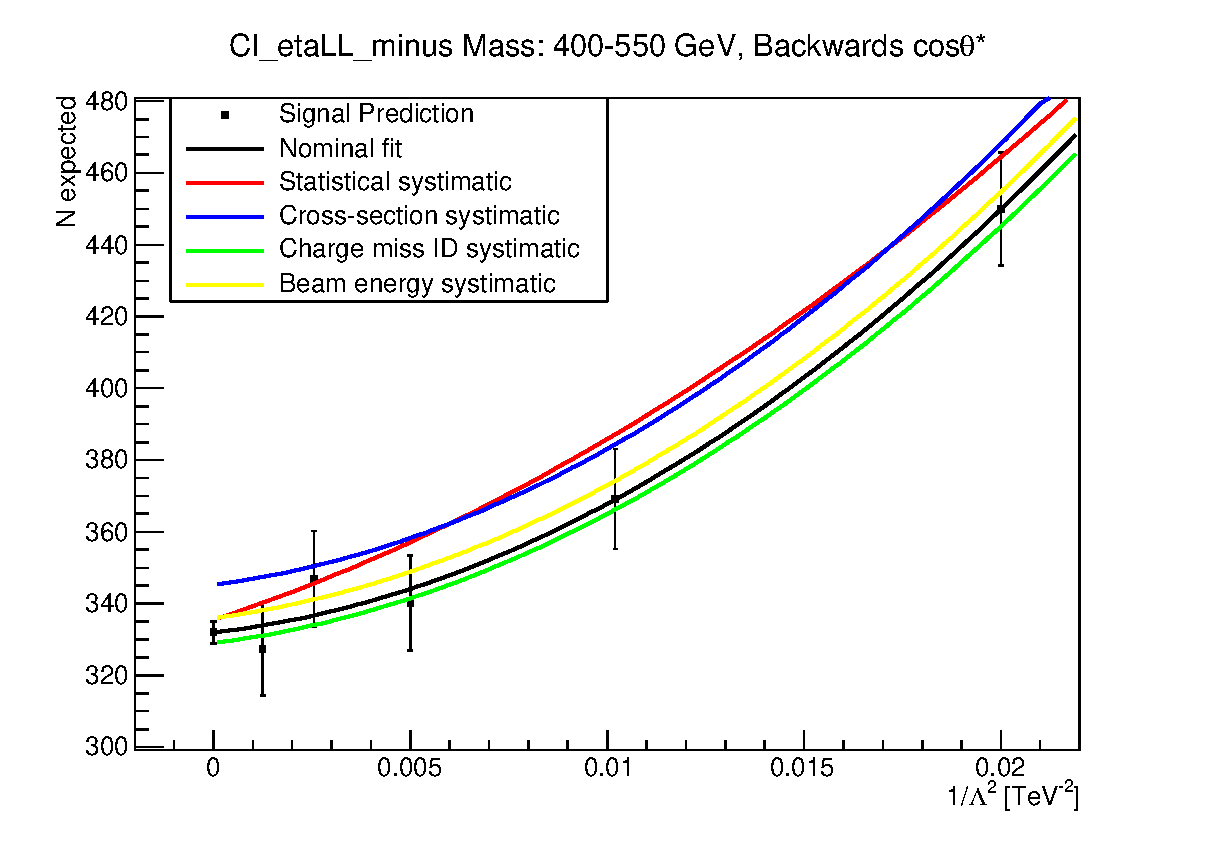
\includegraphics[width=0.49\linewidth]{images/thesis_fits/CI_2D_etaLL_minus_Mass_400-550_GeV_CTS_-1_0.eps}
			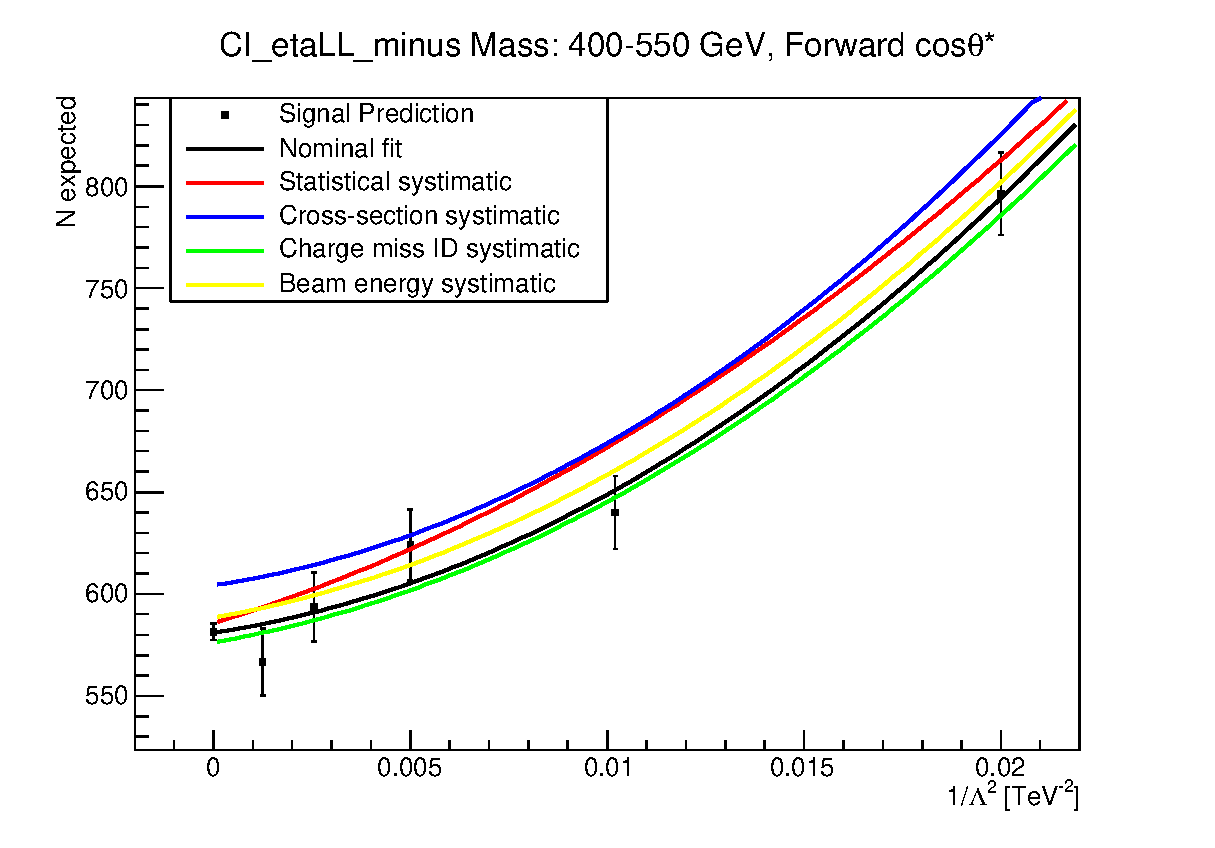
\includegraphics[width=0.49\linewidth]{images/thesis_fits/CI_2D_etaLL_minus_Mass_400-550_GeV_CTS_0_1.eps}
			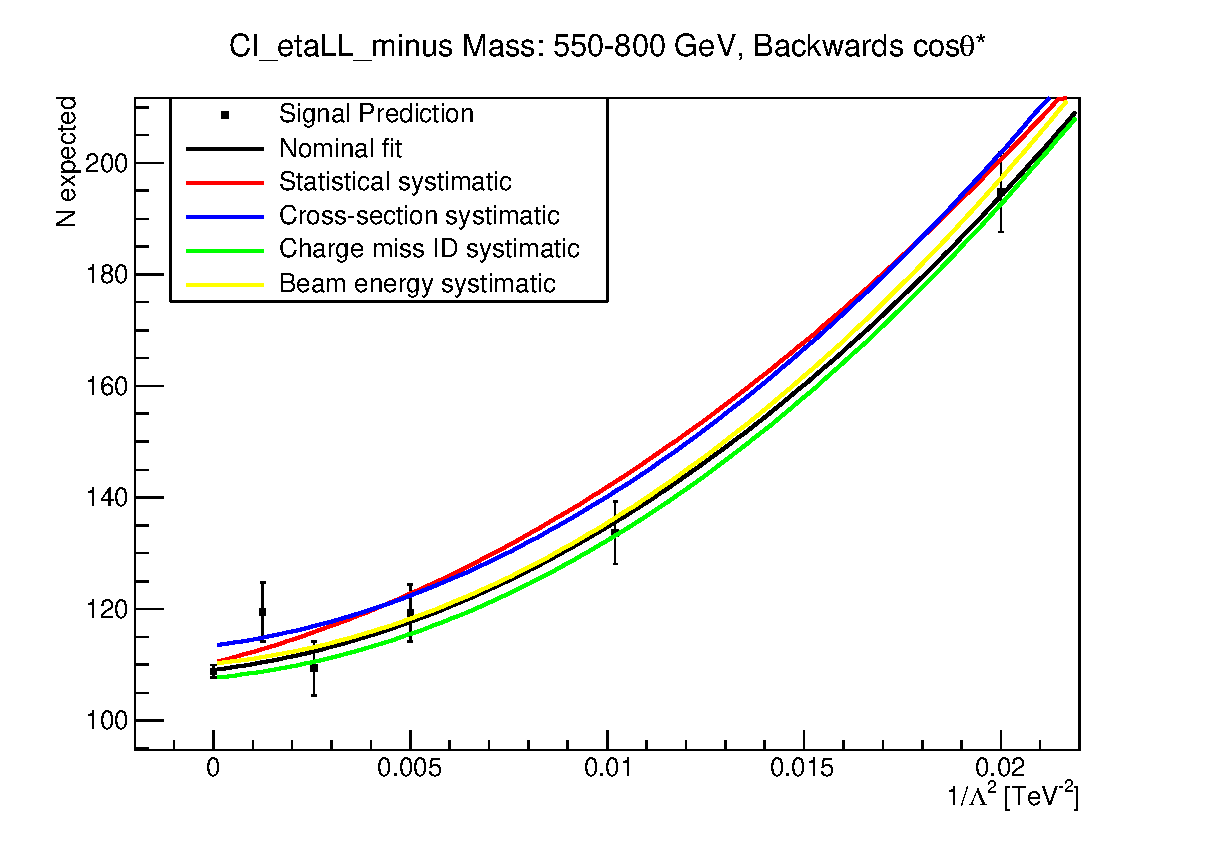
\includegraphics[width=0.49\linewidth]{images/thesis_fits/CI_2D_etaLL_minus_Mass_550-800_GeV_CTS_-1_0.eps}
			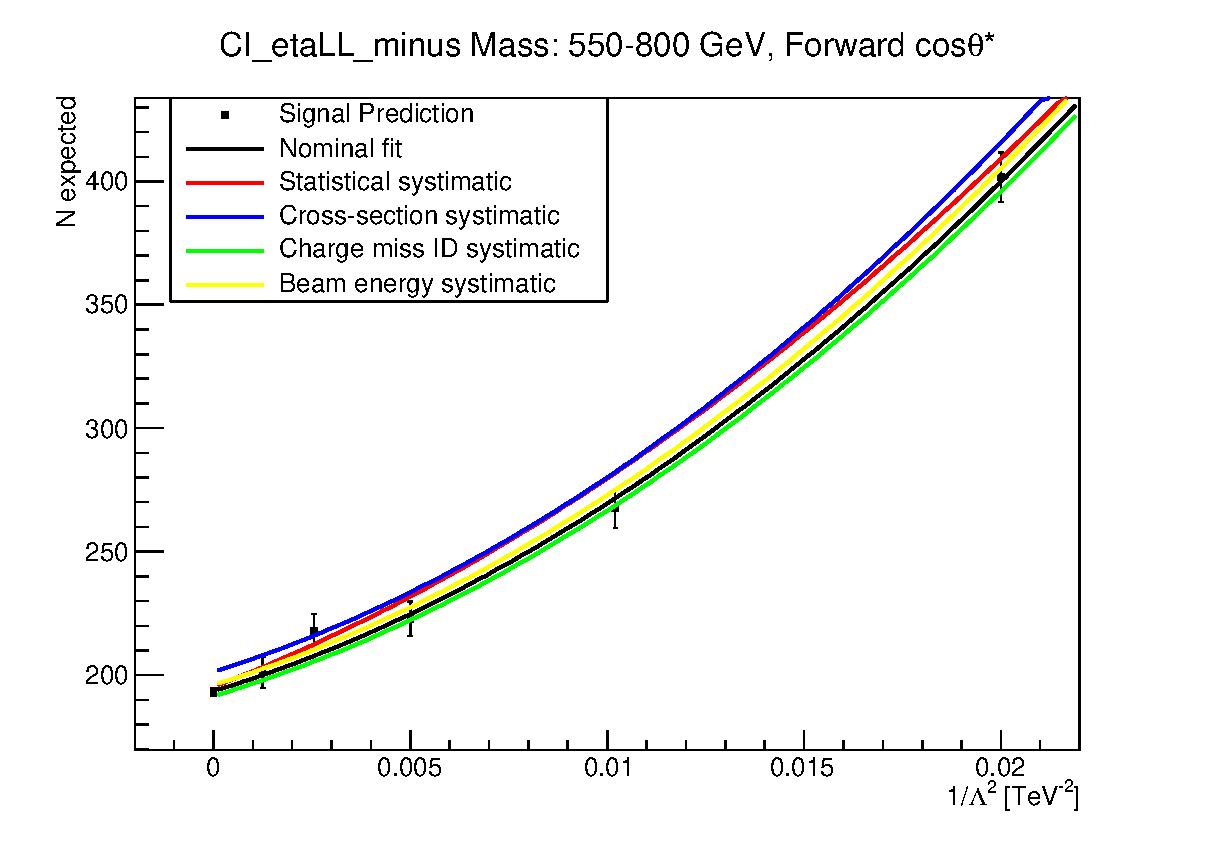
\includegraphics[width=0.49\linewidth]{images/thesis_fits/CI_2D_etaLL_minus_Mass_550-800_GeV_CTS_0_1.eps}
			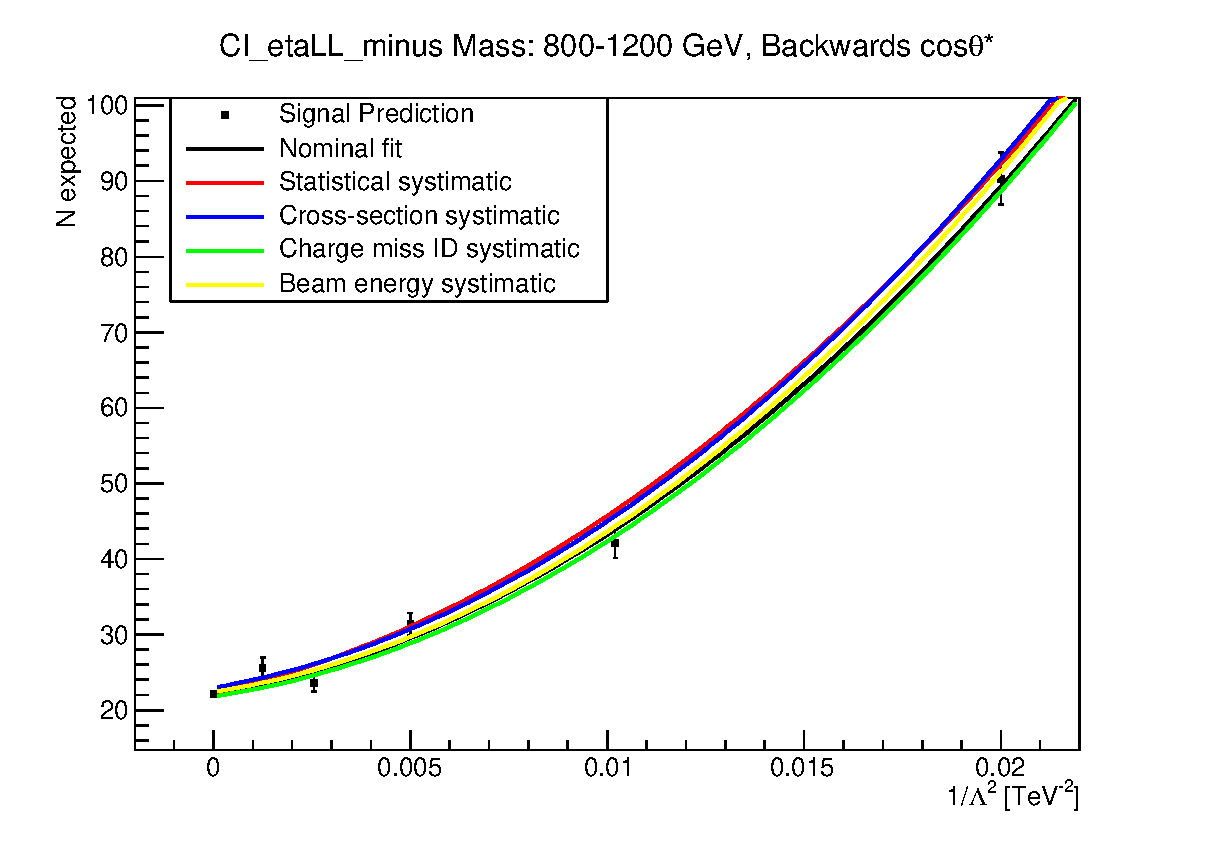
\includegraphics[width=0.49\linewidth]{images/thesis_fits/CI_2D_etaLL_minus_Mass_800-1200_GeV_CTS_-1_0.eps}
			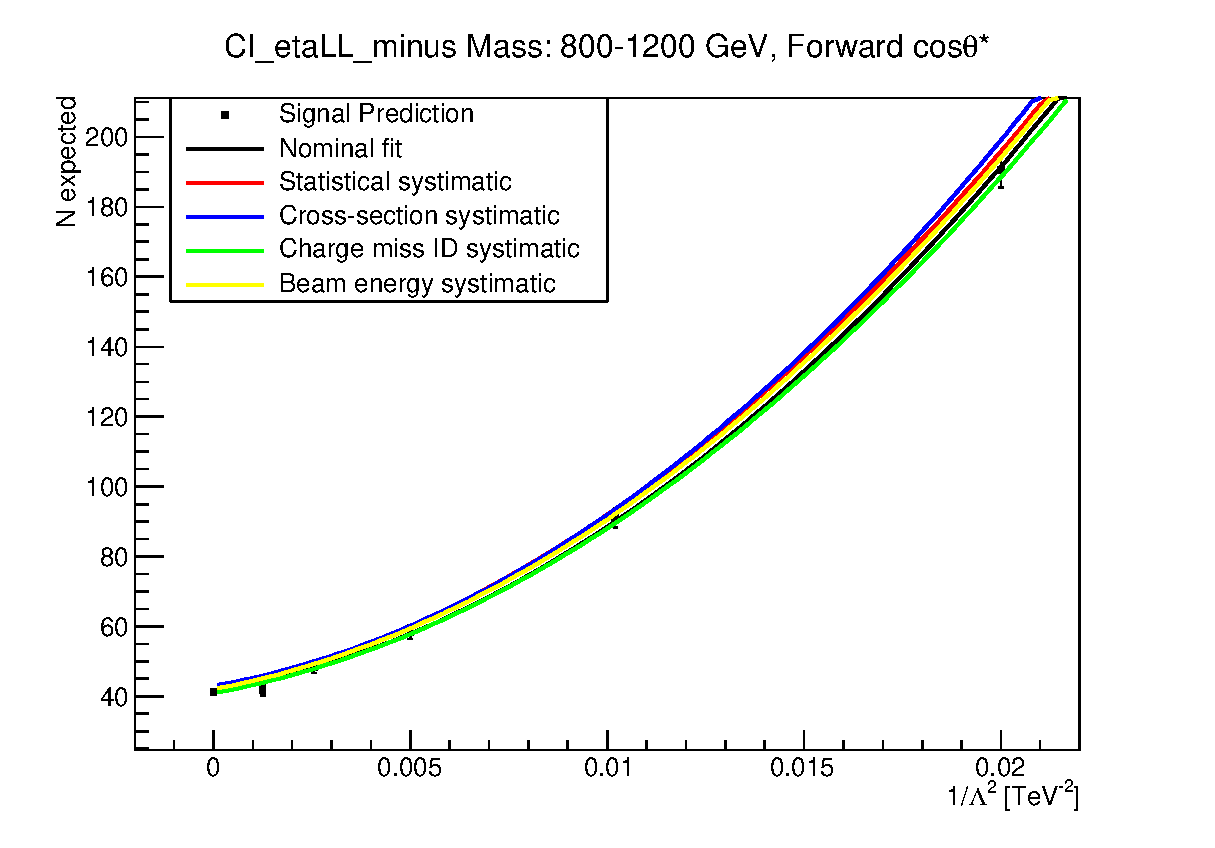
\includegraphics[width=0.49\linewidth]{images/thesis_fits/CI_2D_etaLL_minus_Mass_800-1200_GeV_CTS_0_1.eps}
		\caption{Signal paramaterisations for the LL formalism with constructive interferences for low mass bins}
		\label{fig:parm_LL_m_1}
	\end{figure}

	\begin{figure}[ht]
		\centering
			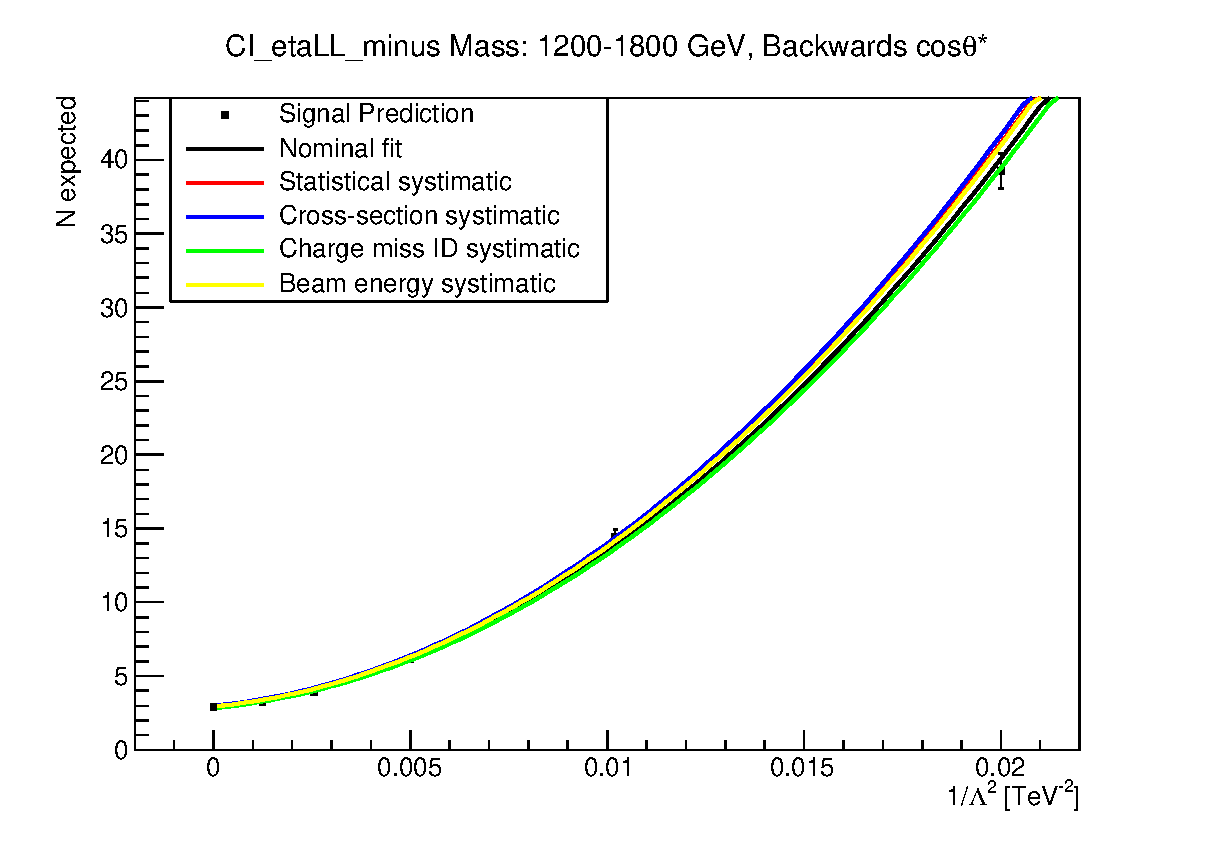
\includegraphics[width=0.49\linewidth]{images/thesis_fits/CI_2D_etaLL_minus_Mass_1200-1800_GeV_CTS_-1_0.eps}
			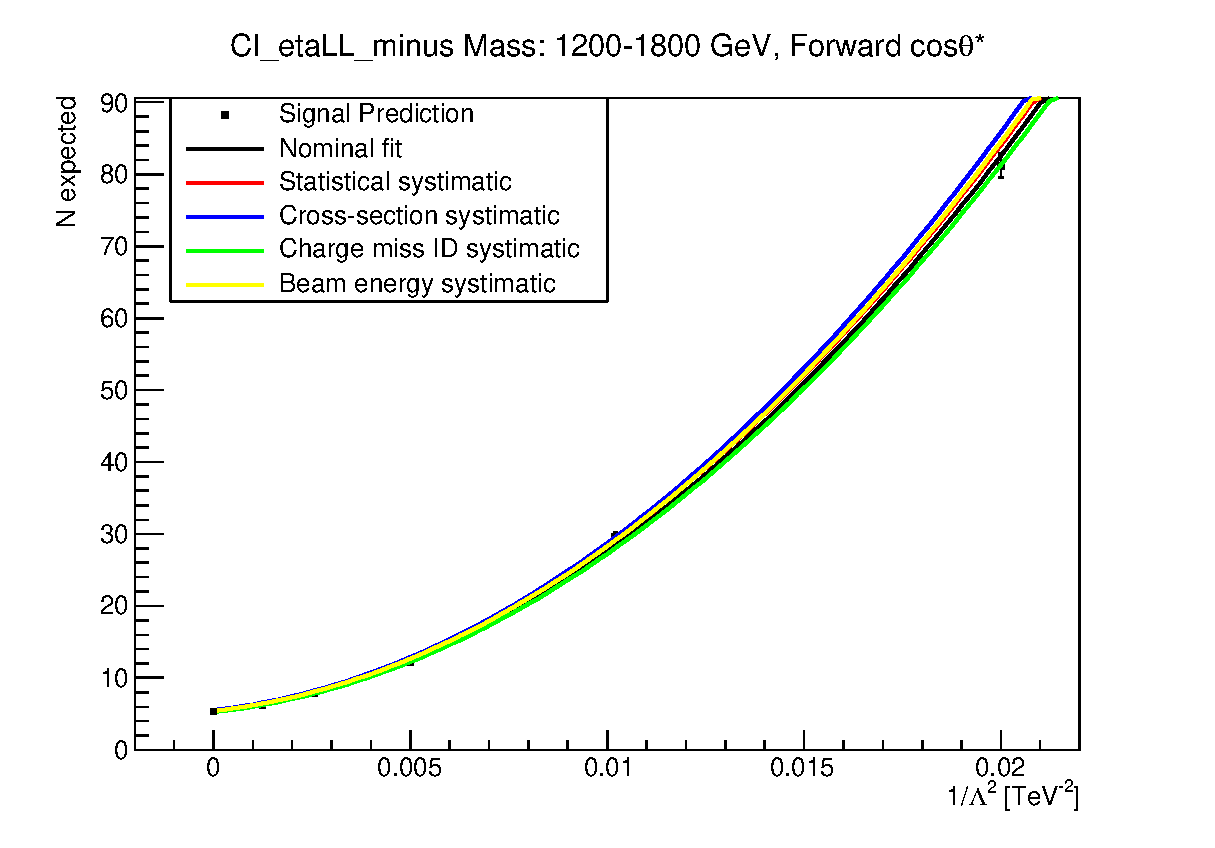
\includegraphics[width=0.49\linewidth]{images/thesis_fits/CI_2D_etaLL_minus_Mass_1200-1800_GeV_CTS_0_1.eps}
			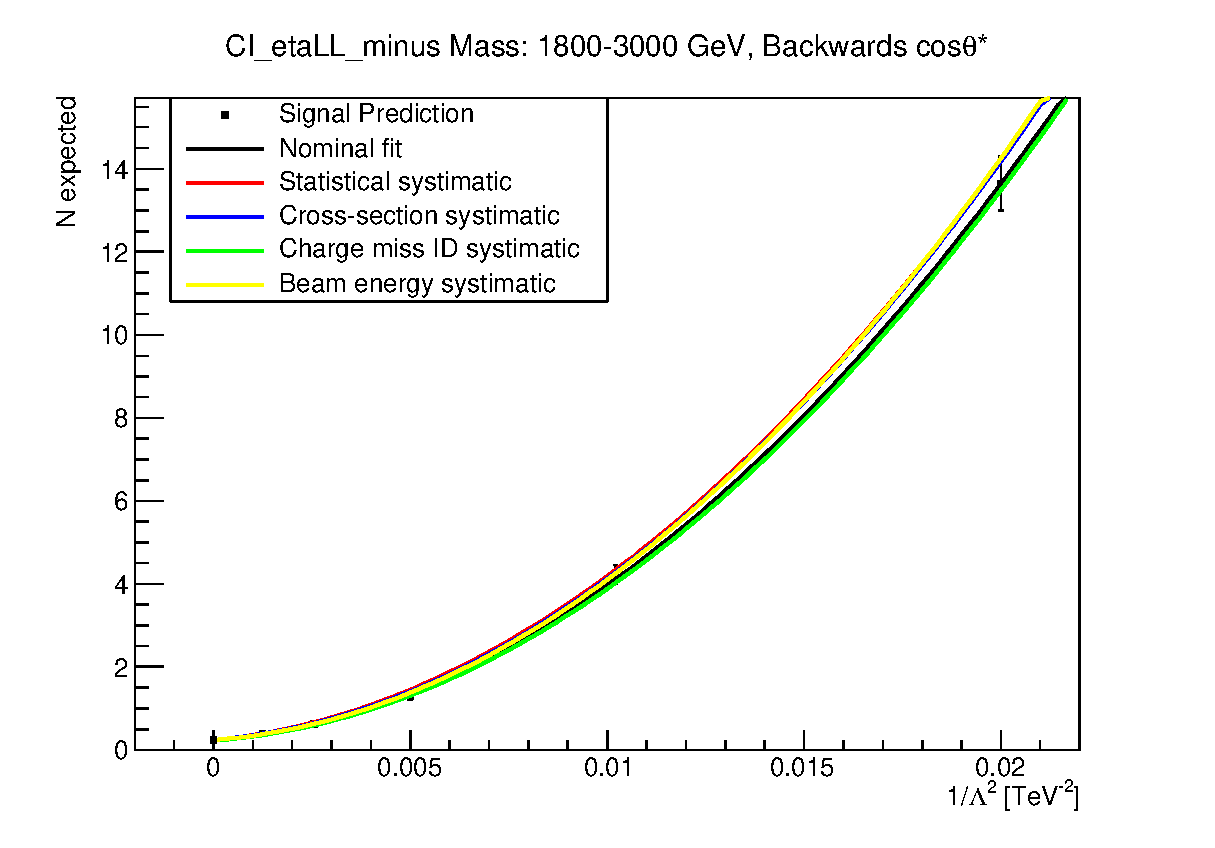
\includegraphics[width=0.49\linewidth]{images/thesis_fits/CI_2D_etaLL_minus_Mass_1800-3000_GeV_CTS_-1_0.eps}
			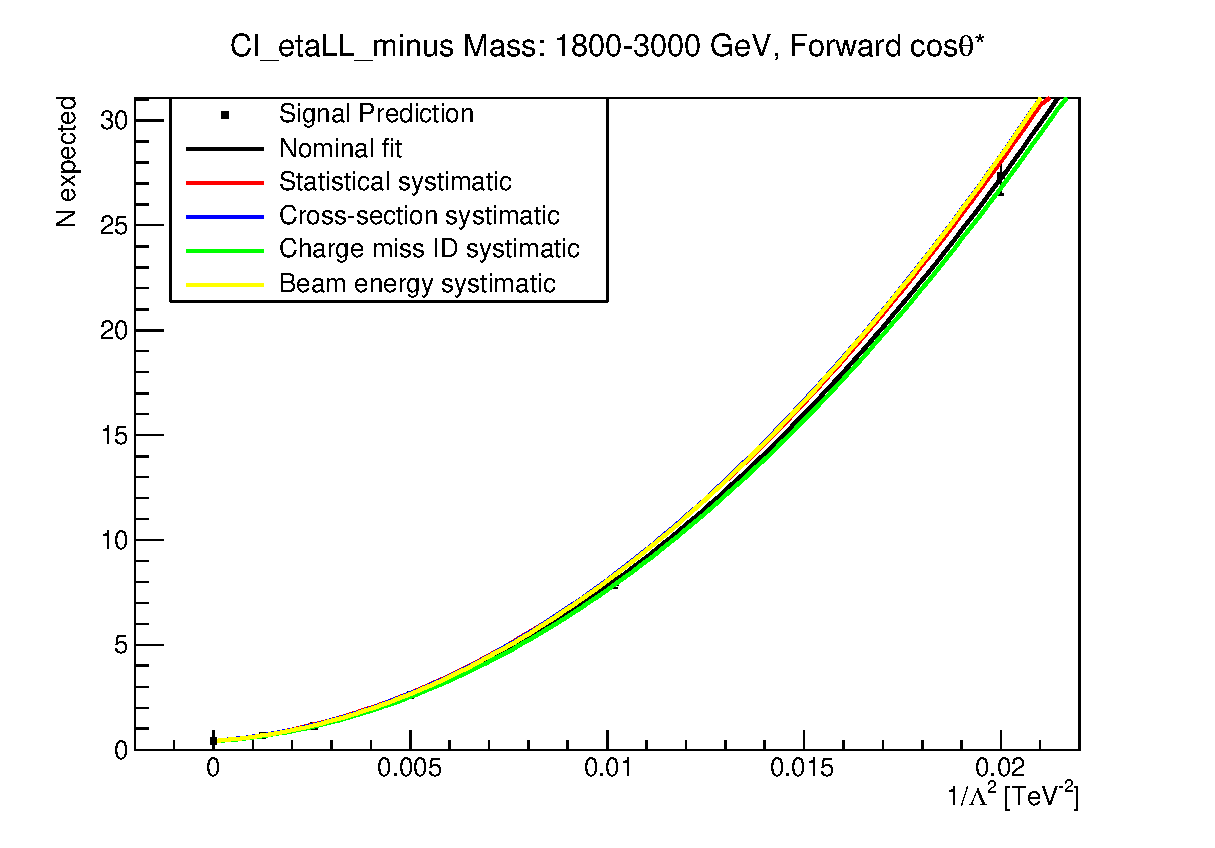
\includegraphics[width=0.49\linewidth]{images/thesis_fits/CI_2D_etaLL_minus_Mass_1800-3000_GeV_CTS_0_1.eps}
			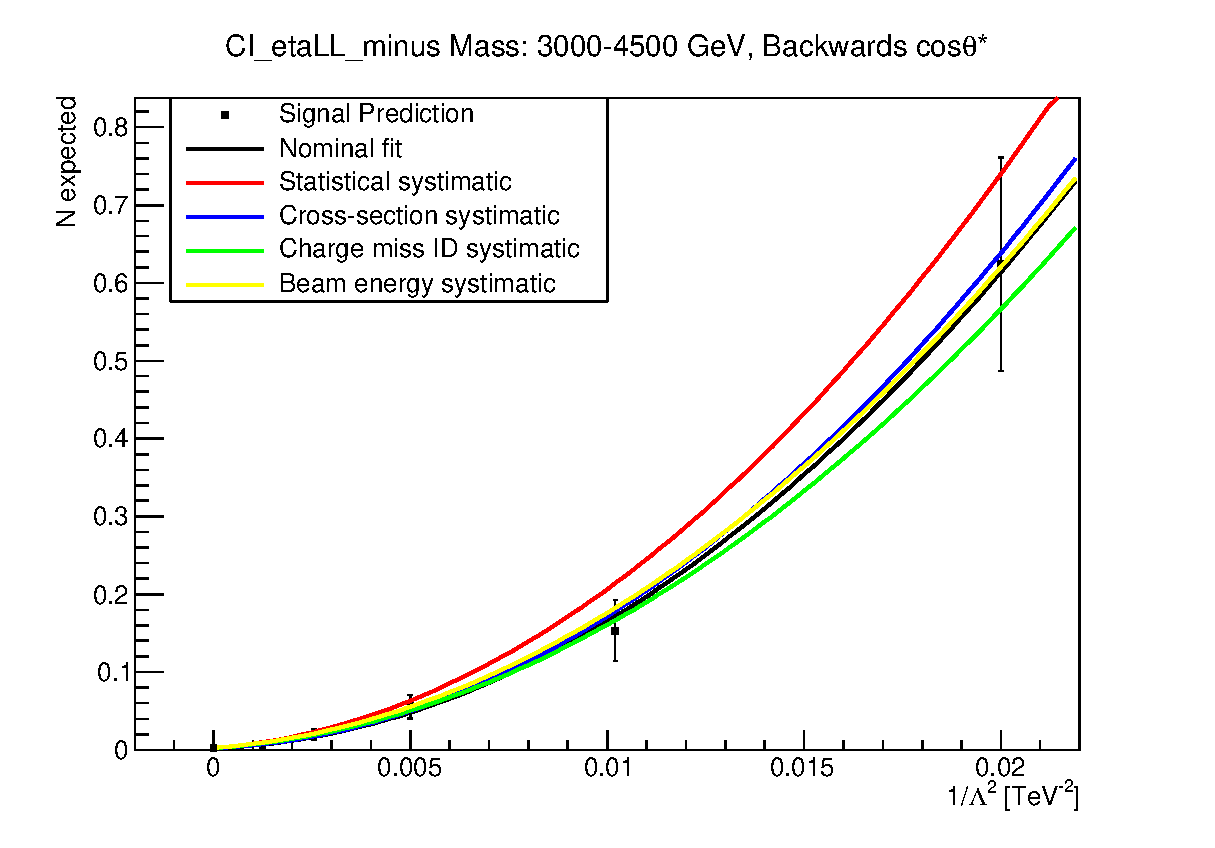
\includegraphics[width=0.49\linewidth]{images/thesis_fits/CI_2D_etaLL_minus_Mass_3000-4500_GeV_CTS_-1_0.eps}
			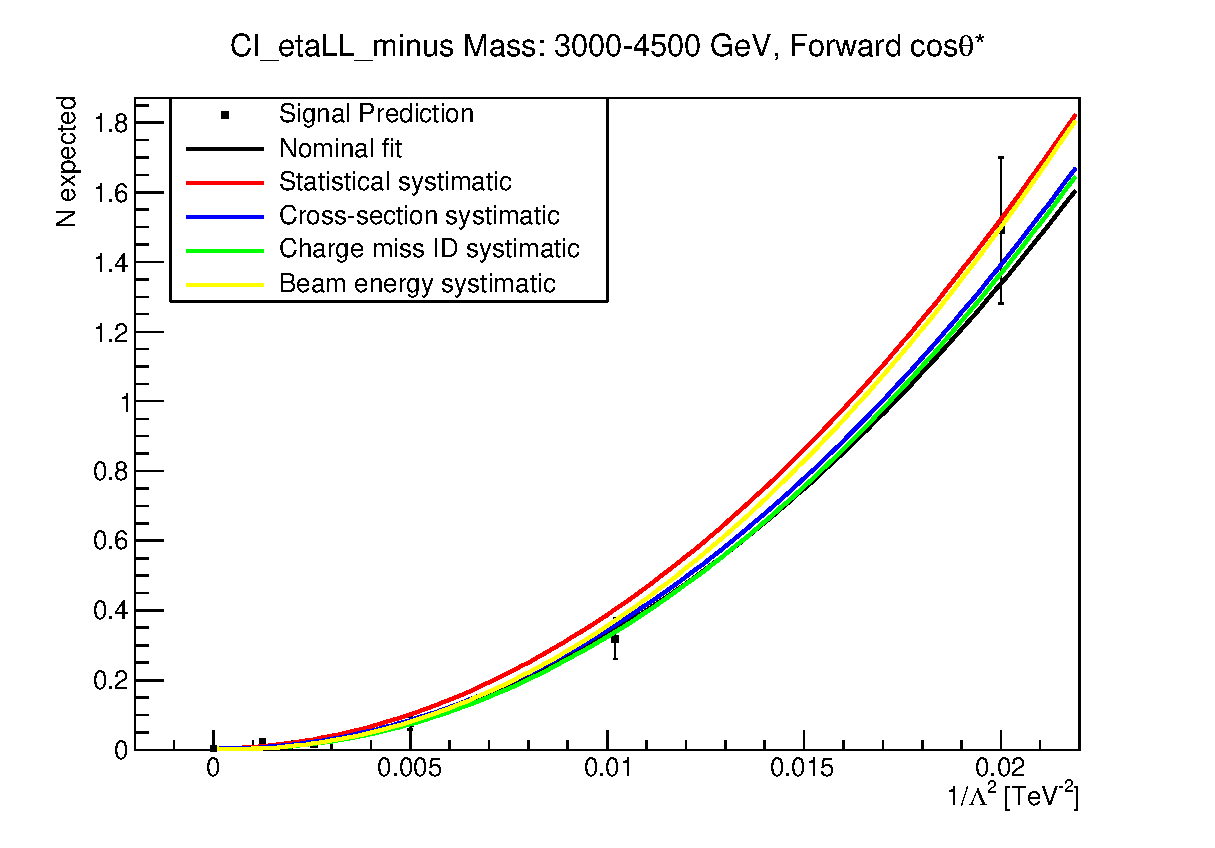
\includegraphics[width=0.49\linewidth]{images/thesis_fits/CI_2D_etaLL_minus_Mass_3000-4500_GeV_CTS_0_1.eps}
		\caption{Signal paramaterisations for the LL formalism with constructive interferences for high mass bins}
		\label{fig:parm_LL_m_2}
	\end{figure}


	\begin{figure}[ht]
		\centering
			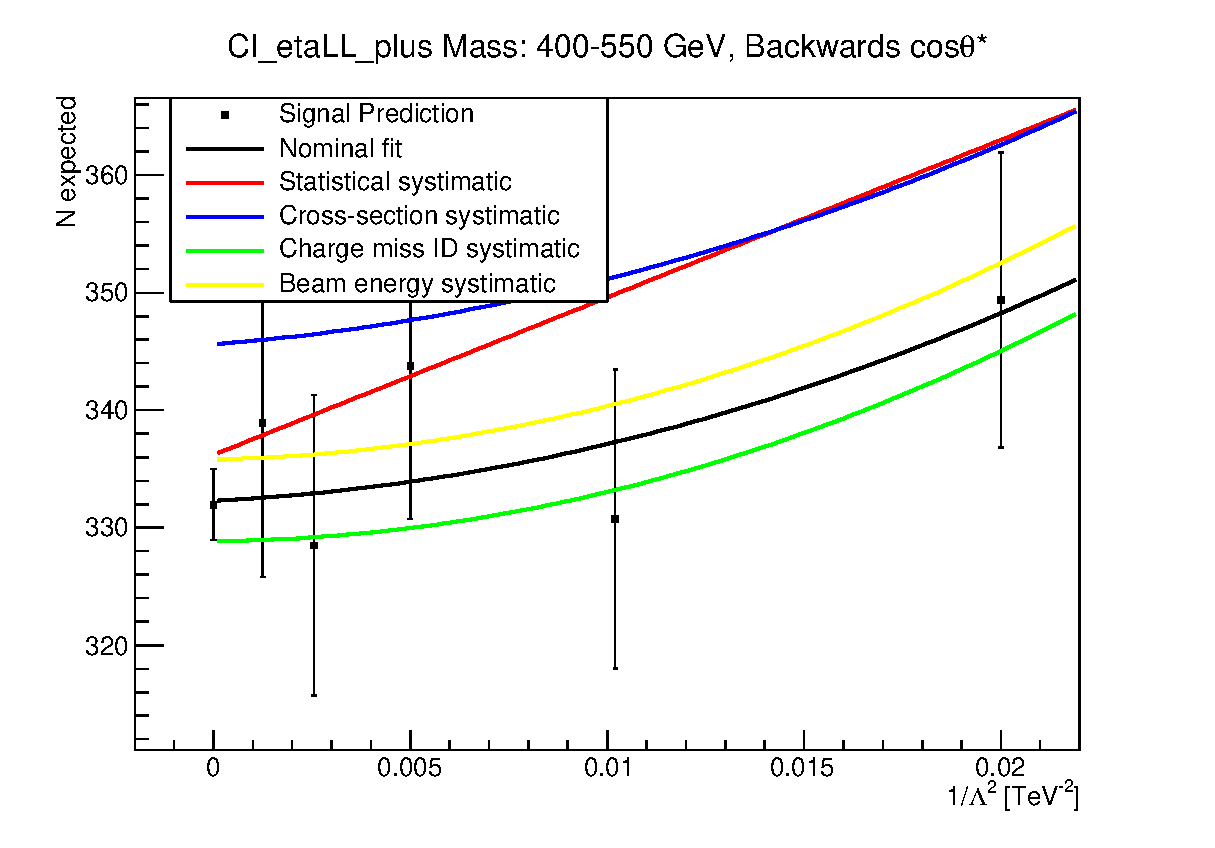
\includegraphics[width=0.49\linewidth]{images/thesis_fits/CI_2D_etaLL_plus_Mass_400-550_GeV_CTS_-1_0.eps}
			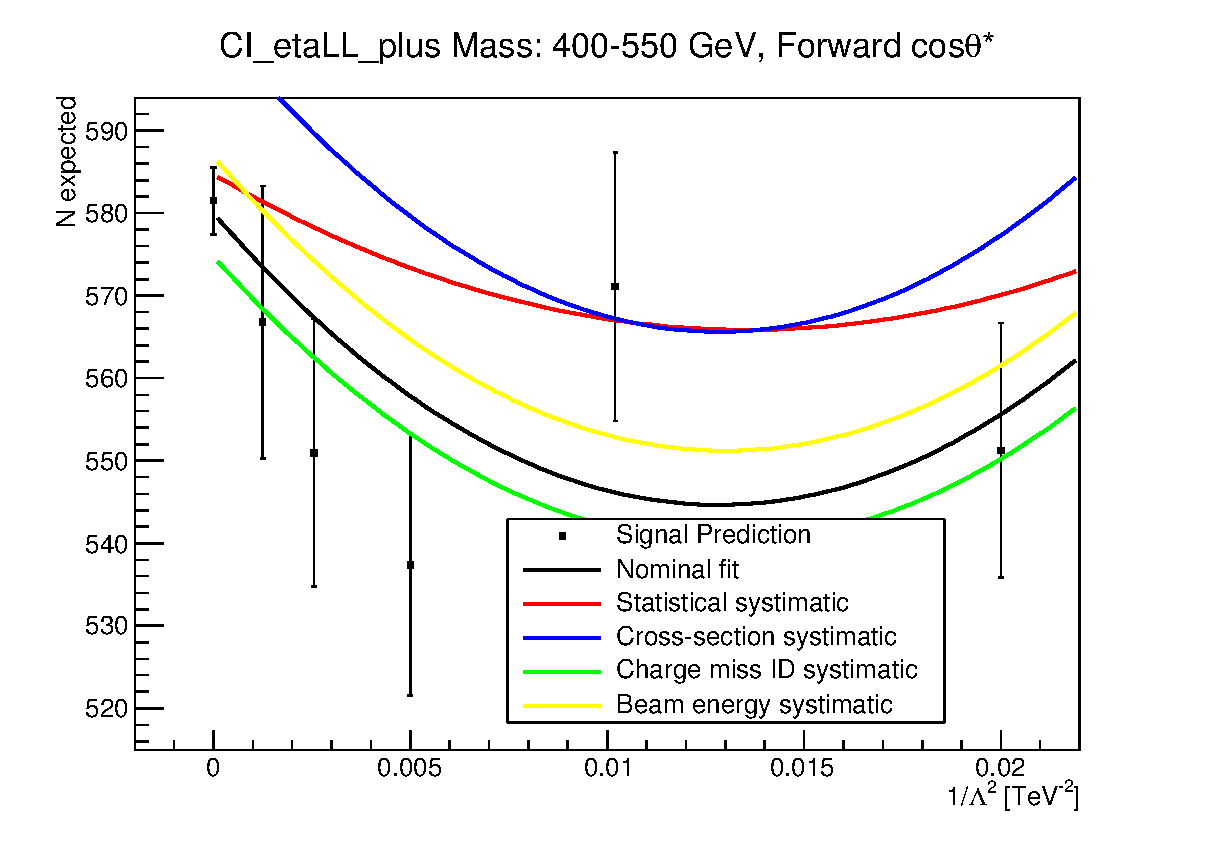
\includegraphics[width=0.49\linewidth]{images/thesis_fits/CI_2D_etaLL_plus_Mass_400-550_GeV_CTS_0_1.eps}
			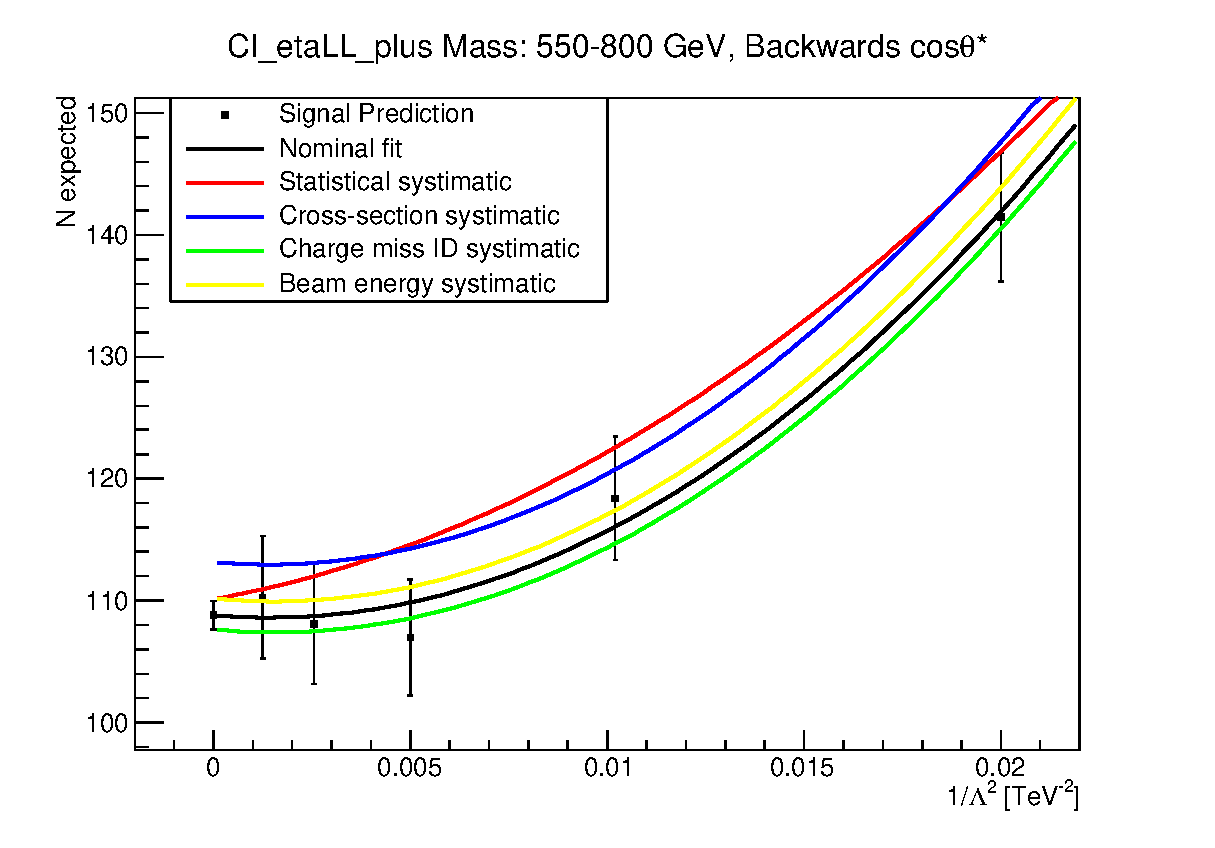
\includegraphics[width=0.49\linewidth]{images/thesis_fits/CI_2D_etaLL_plus_Mass_550-800_GeV_CTS_-1_0.eps}
			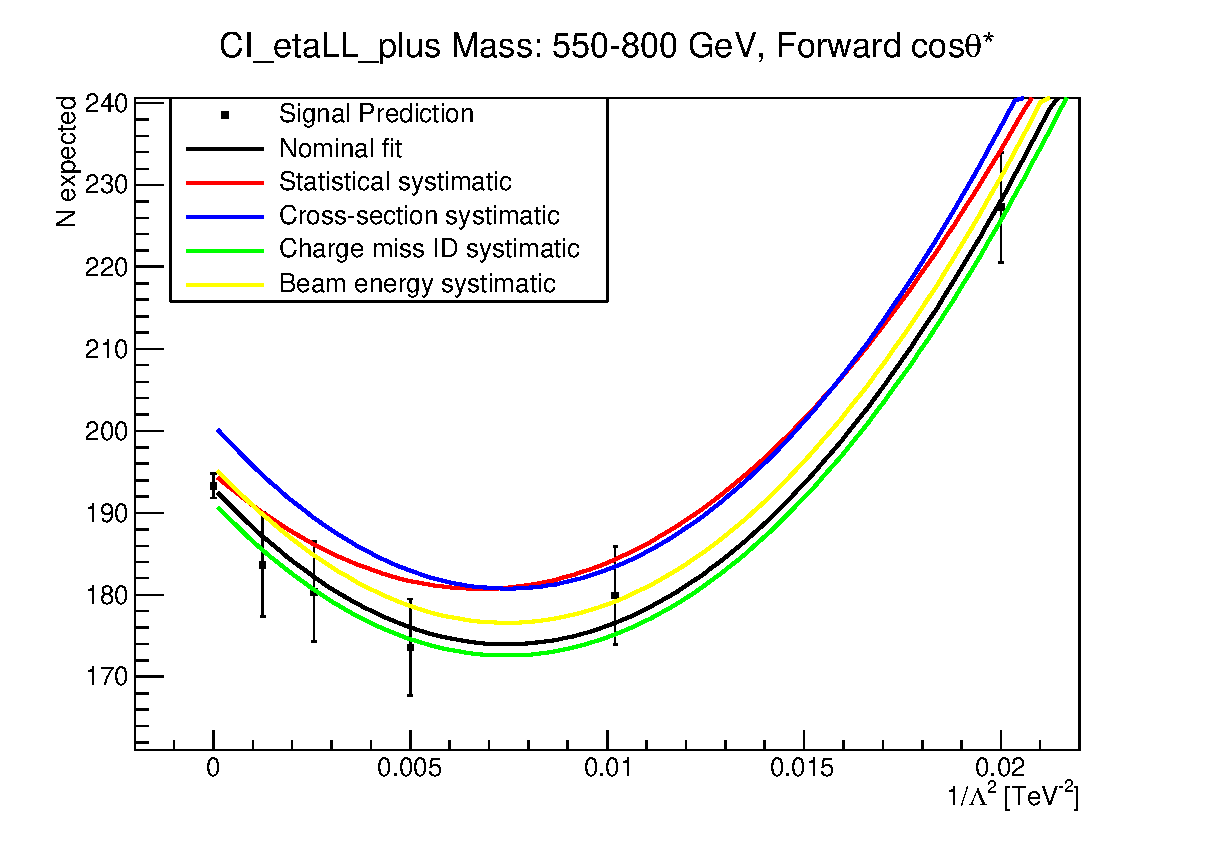
\includegraphics[width=0.49\linewidth]{images/thesis_fits/CI_2D_etaLL_plus_Mass_550-800_GeV_CTS_0_1.eps}
			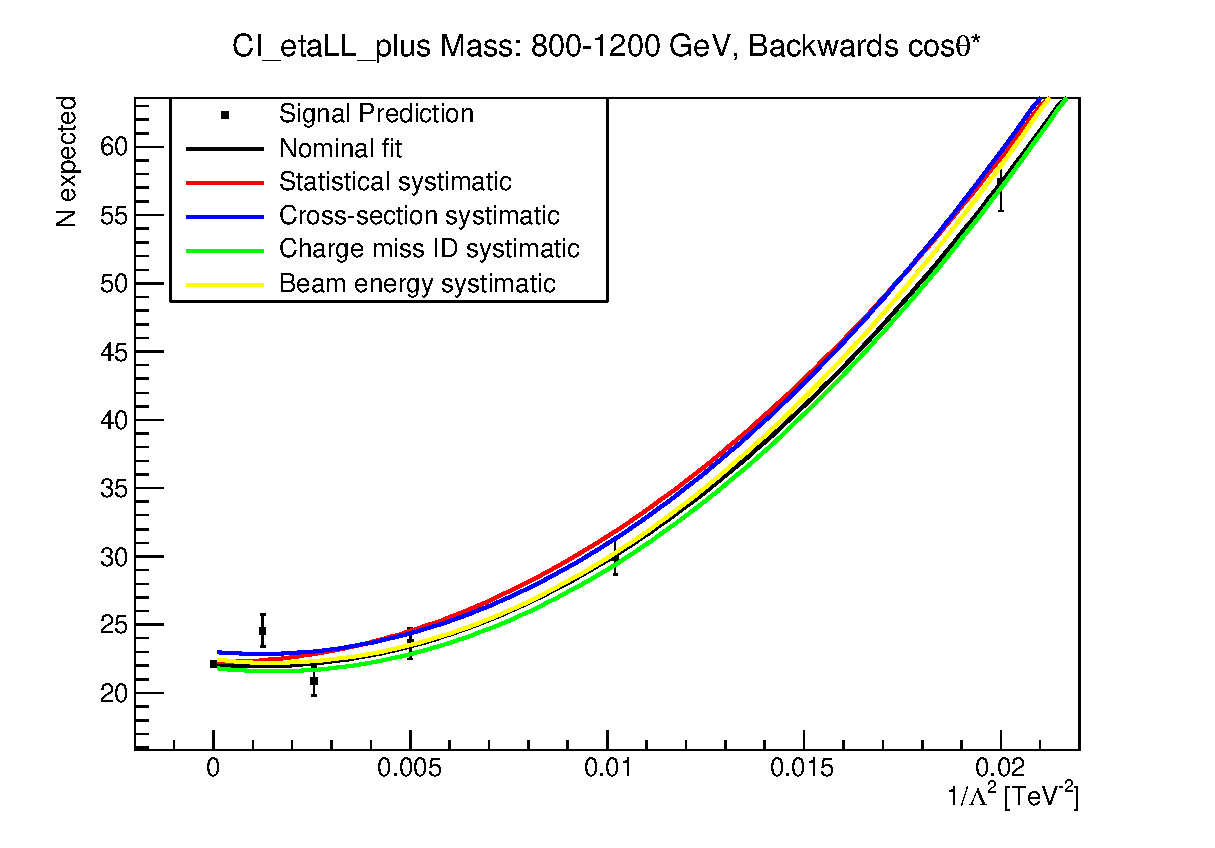
\includegraphics[width=0.49\linewidth]{images/thesis_fits/CI_2D_etaLL_plus_Mass_800-1200_GeV_CTS_-1_0.eps}
			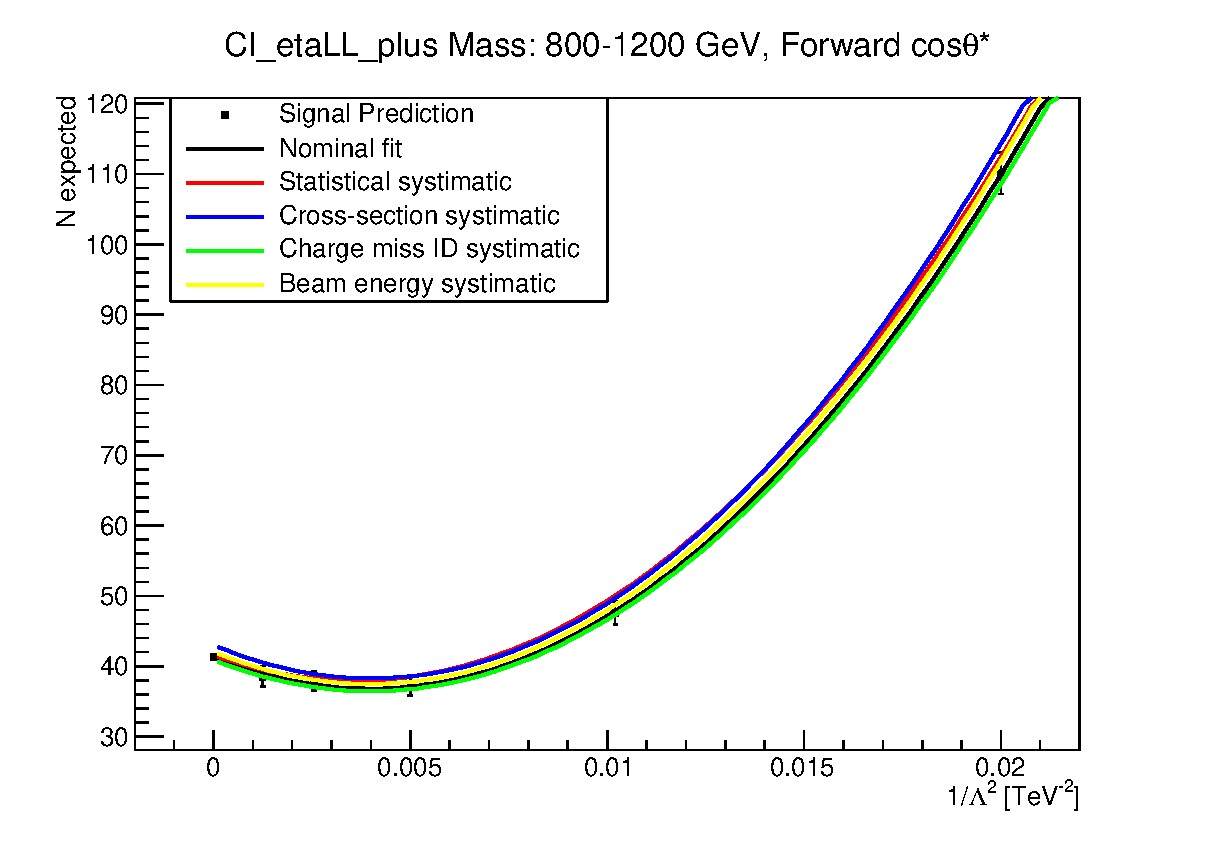
\includegraphics[width=0.49\linewidth]{images/thesis_fits/CI_2D_etaLL_plus_Mass_800-1200_GeV_CTS_0_1.eps}
		\caption{Signal paramaterisations for the LL formalism with destructive interferences for low mass bins}
		\label{fig:parm_LL_p_1}
	\end{figure}

	\begin{figure}[ht]
		\centering
			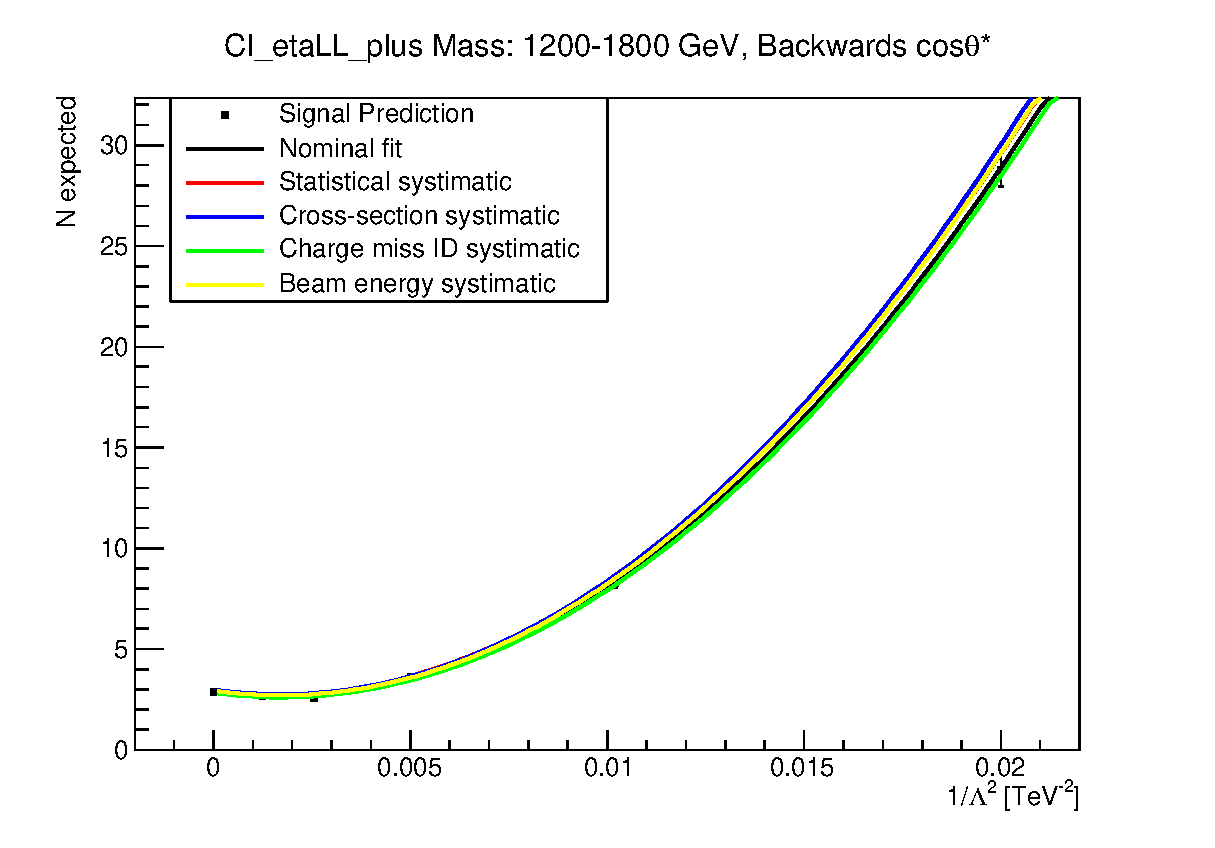
\includegraphics[width=0.49\linewidth]{images/thesis_fits/CI_2D_etaLL_plus_Mass_1200-1800_GeV_CTS_-1_0.eps}
			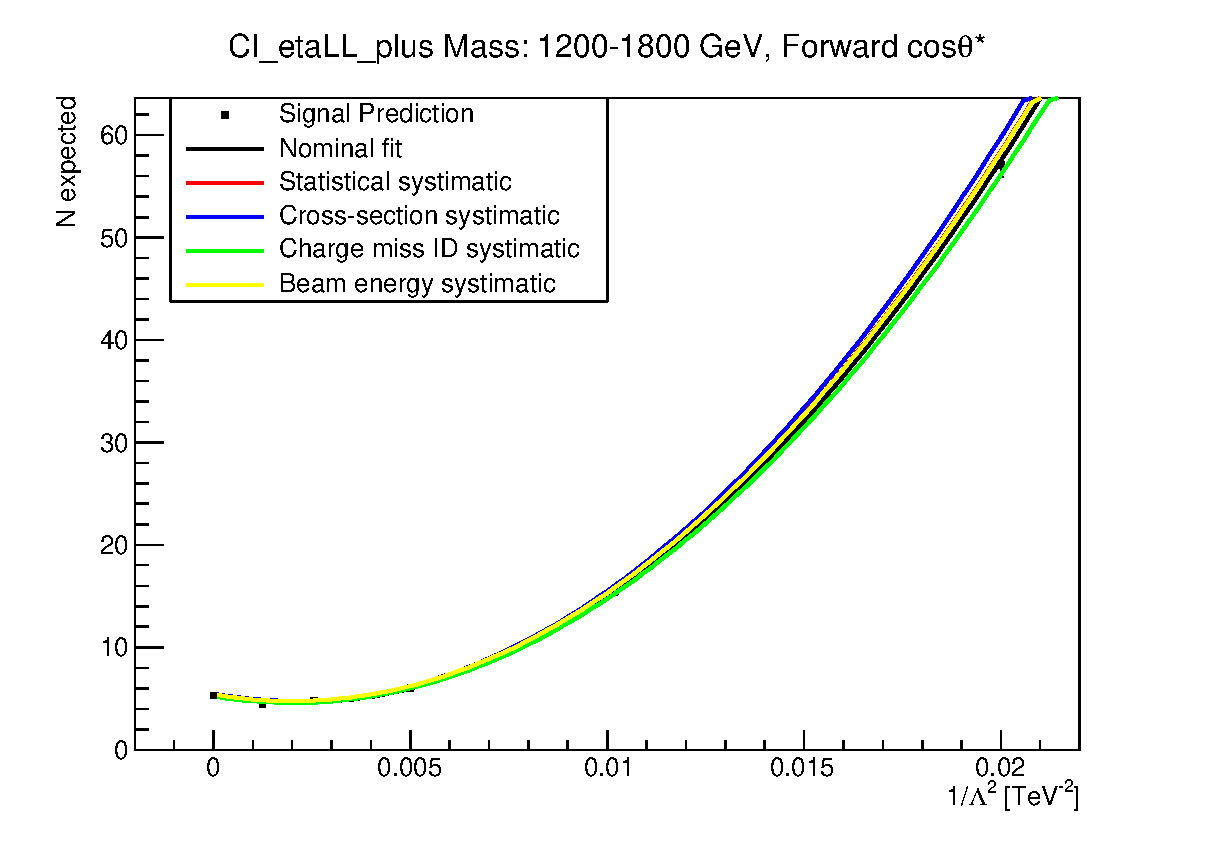
\includegraphics[width=0.49\linewidth]{images/thesis_fits/CI_2D_etaLL_plus_Mass_1200-1800_GeV_CTS_0_1.eps}
			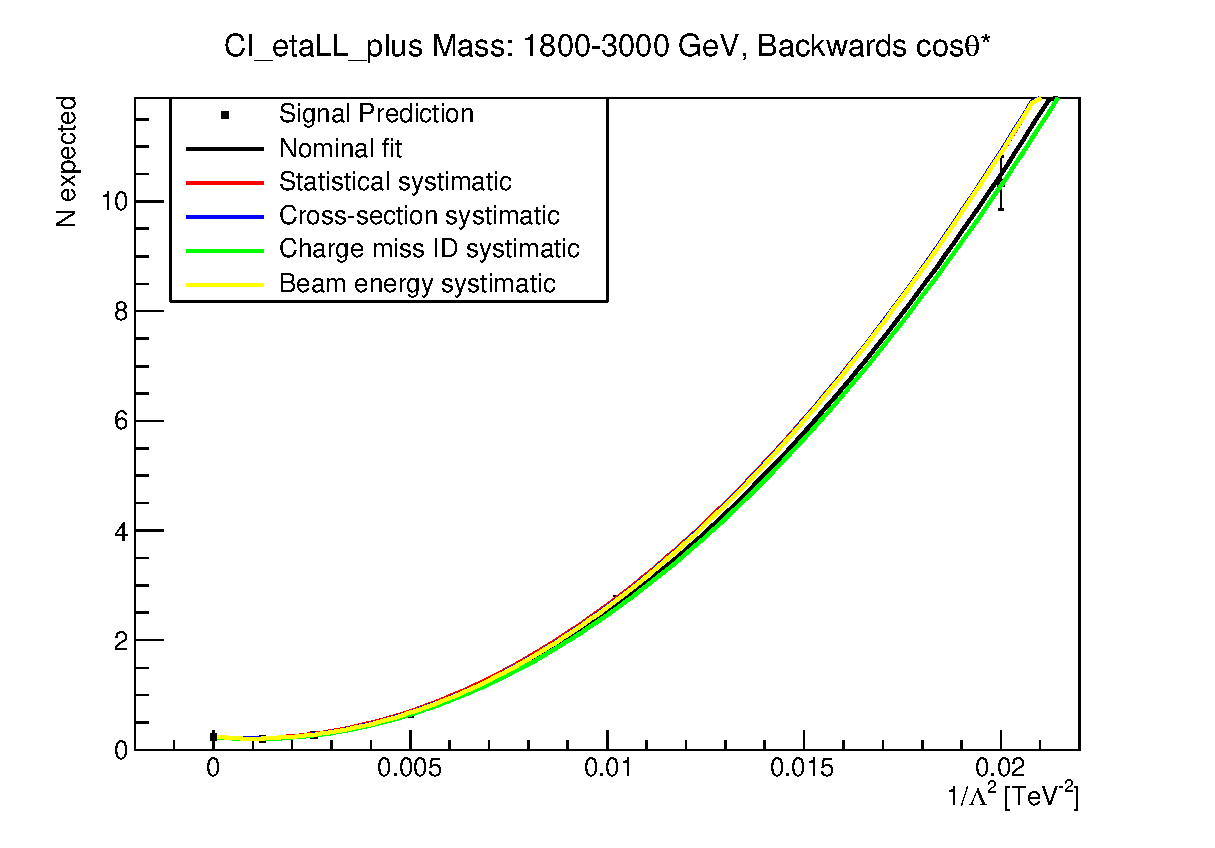
\includegraphics[width=0.49\linewidth]{images/thesis_fits/CI_2D_etaLL_plus_Mass_1800-3000_GeV_CTS_-1_0.eps}
			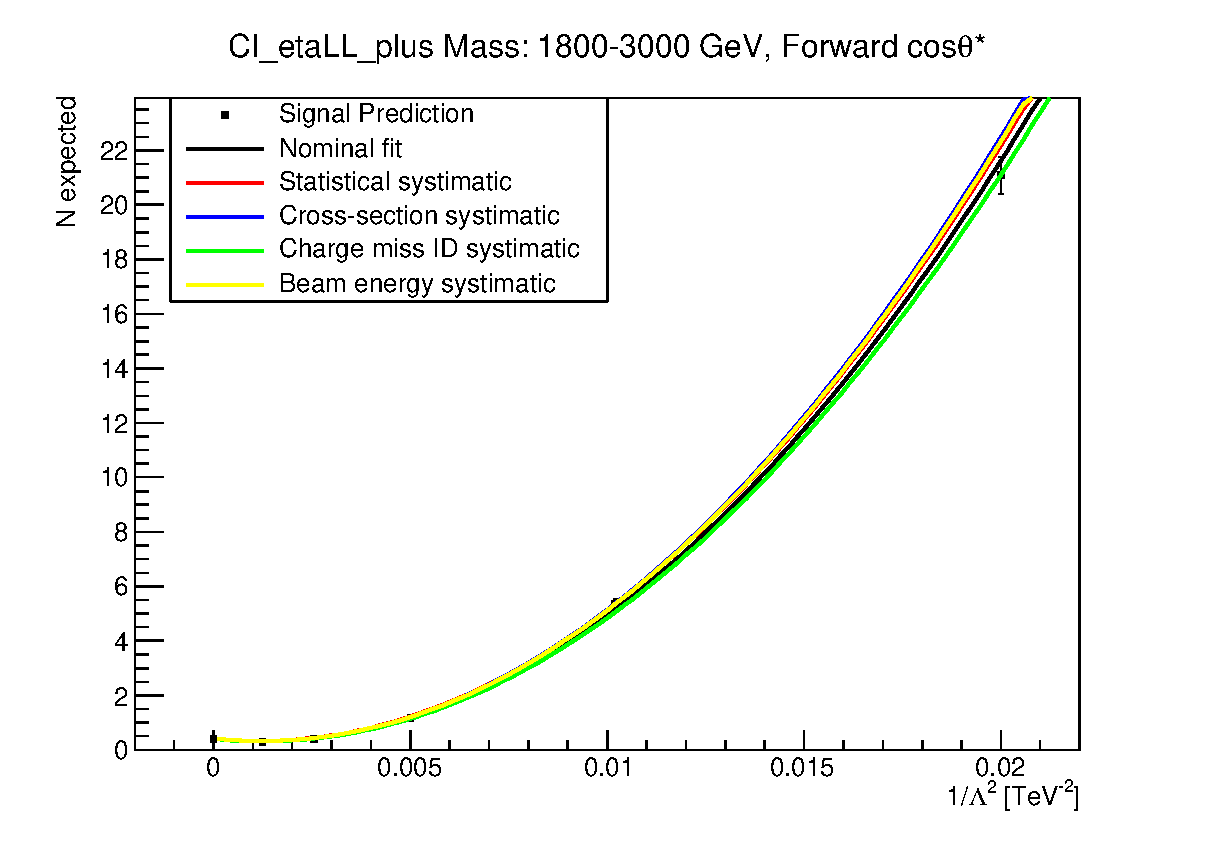
\includegraphics[width=0.49\linewidth]{images/thesis_fits/CI_2D_etaLL_plus_Mass_1800-3000_GeV_CTS_0_1.eps}
			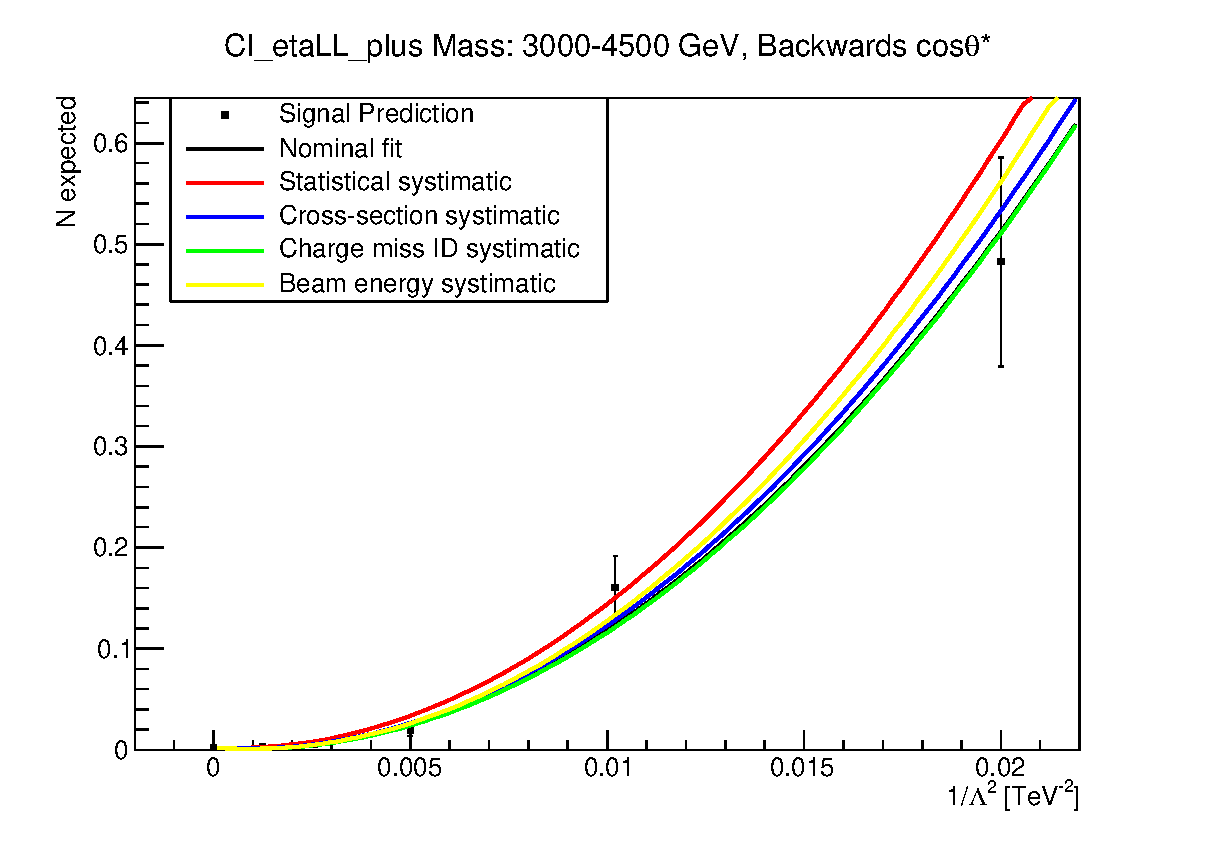
\includegraphics[width=0.49\linewidth]{images/thesis_fits/CI_2D_etaLL_plus_Mass_3000-4500_GeV_CTS_-1_0.eps}
			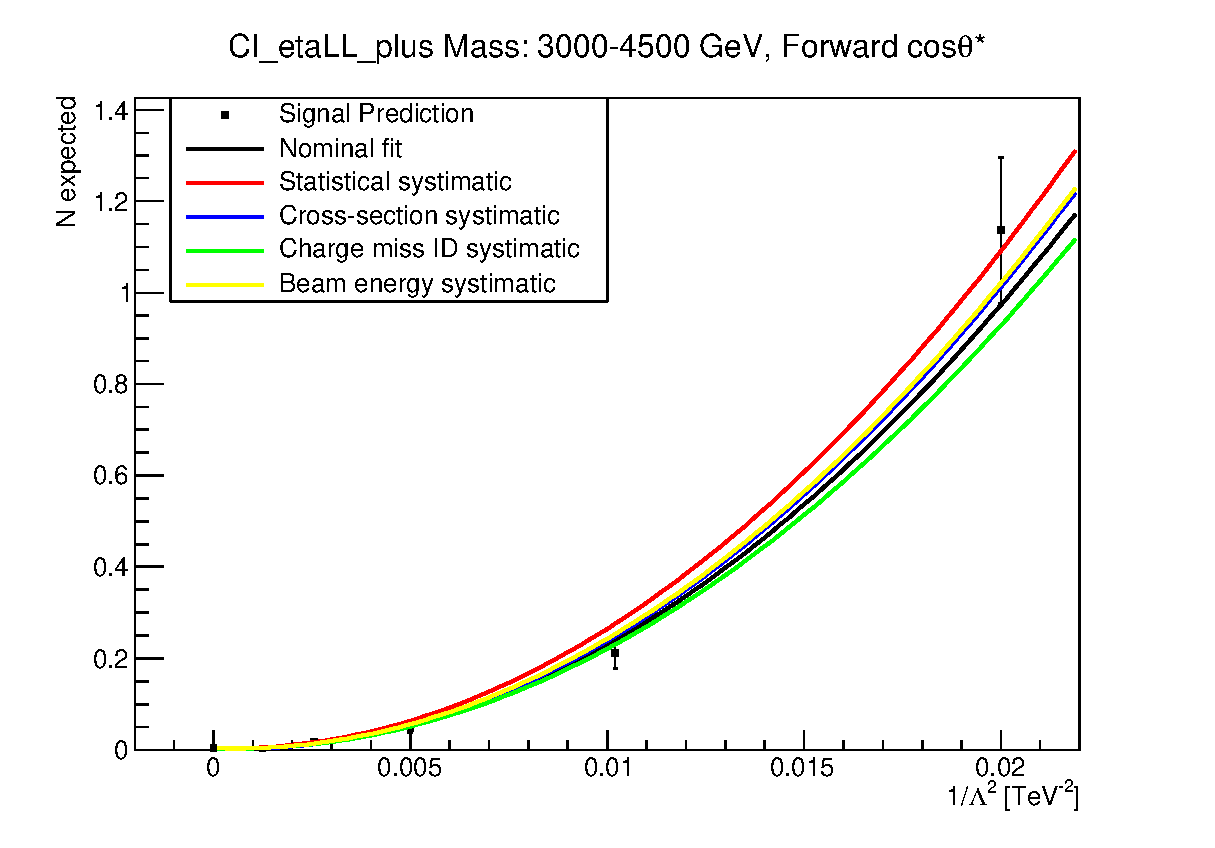
\includegraphics[width=0.49\linewidth]{images/thesis_fits/CI_2D_etaLL_plus_Mass_3000-4500_GeV_CTS_0_1.eps}
		\caption{Signal paramaterisations for the LL formalism with destructive interferences for high mass bins}
		\label{fig:parm_LL_p_2}
	\end{figure}














	\begin{figure}[ht]
		\centering
			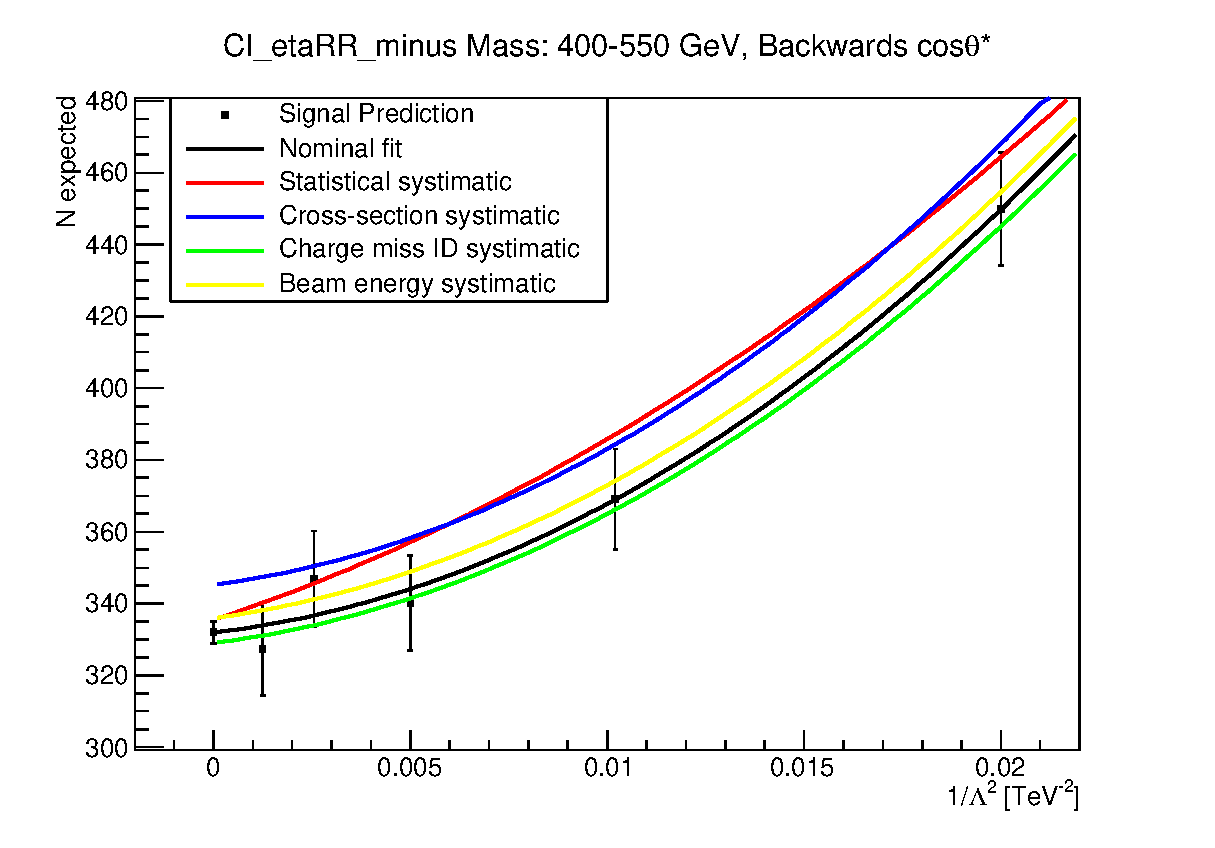
\includegraphics[width=0.49\linewidth]{images/thesis_fits/CI_2D_etaRR_minus_Mass_400-550_GeV_CTS_-1_0.eps}
			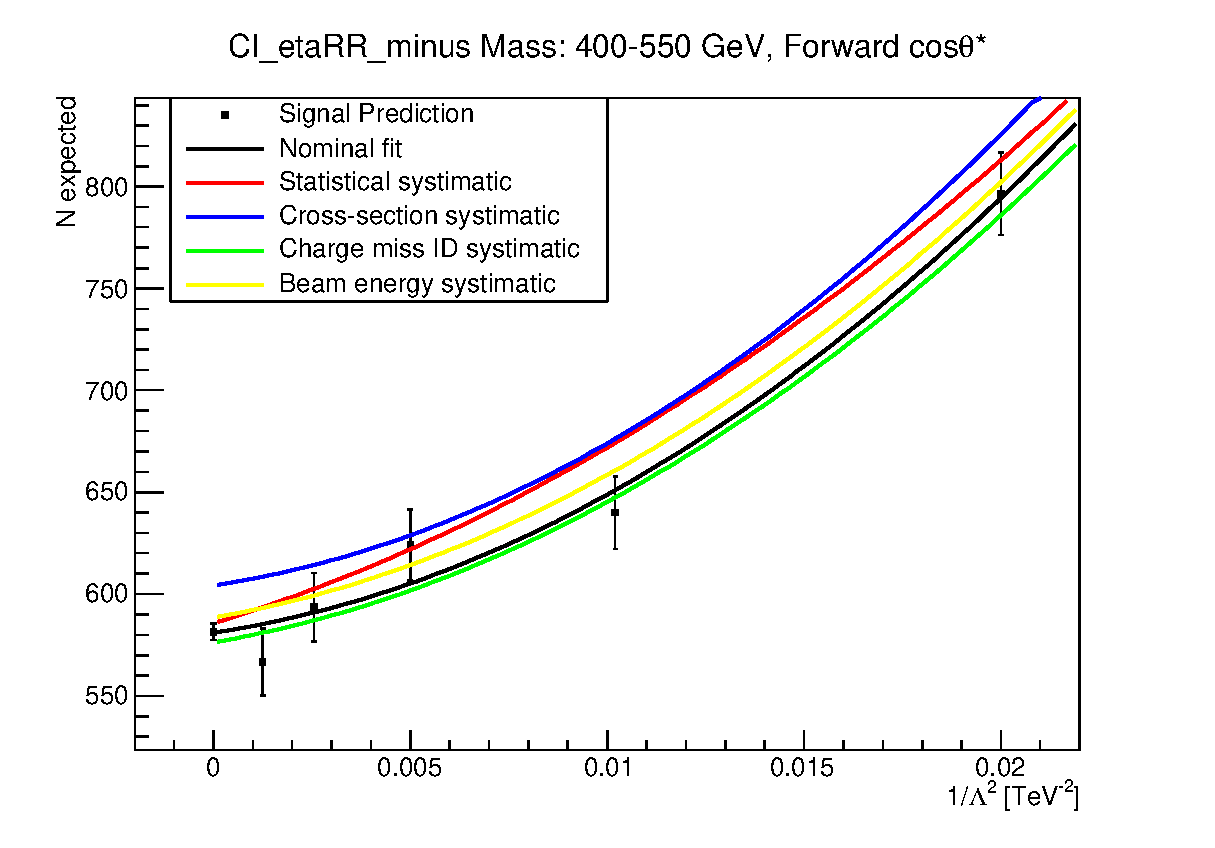
\includegraphics[width=0.49\linewidth]{images/thesis_fits/CI_2D_etaRR_minus_Mass_400-550_GeV_CTS_0_1.eps}
			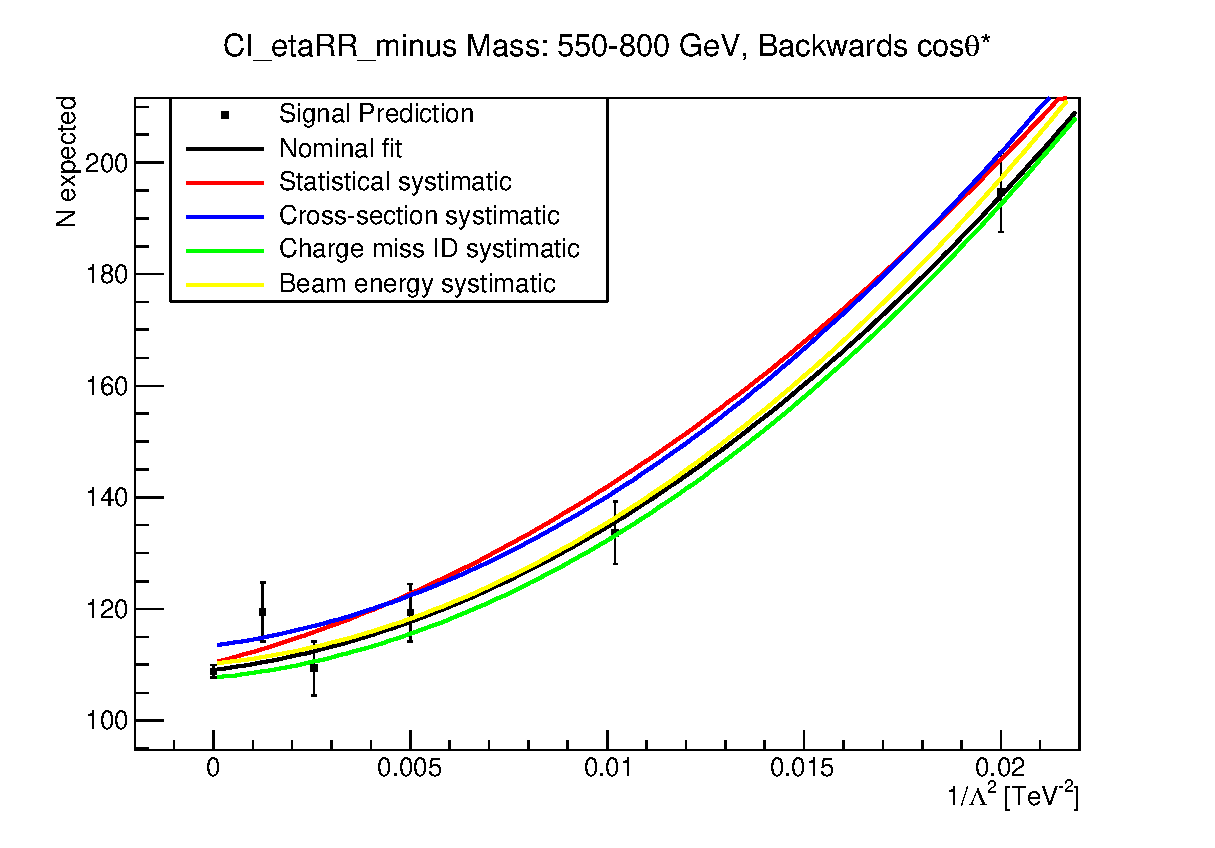
\includegraphics[width=0.49\linewidth]{images/thesis_fits/CI_2D_etaRR_minus_Mass_550-800_GeV_CTS_-1_0.eps}
			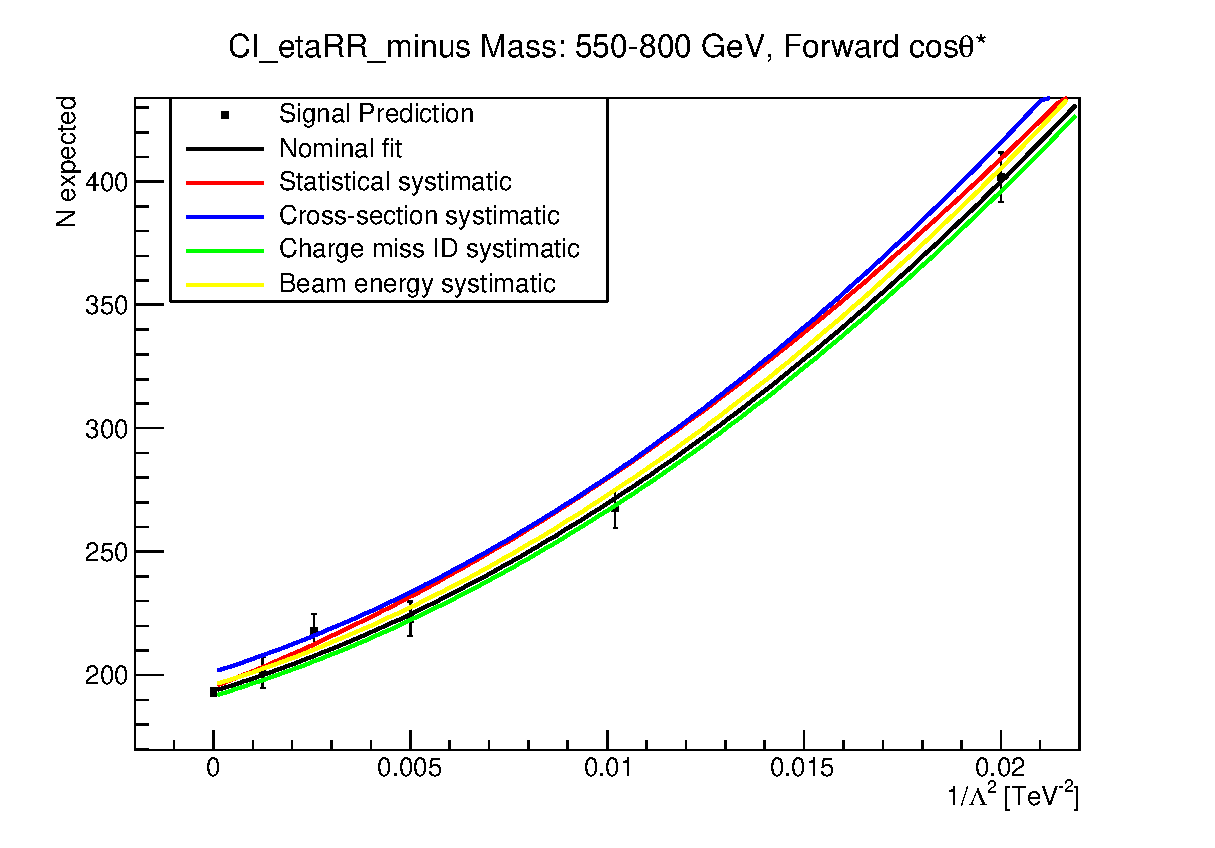
\includegraphics[width=0.49\linewidth]{images/thesis_fits/CI_2D_etaRR_minus_Mass_550-800_GeV_CTS_0_1.eps}
			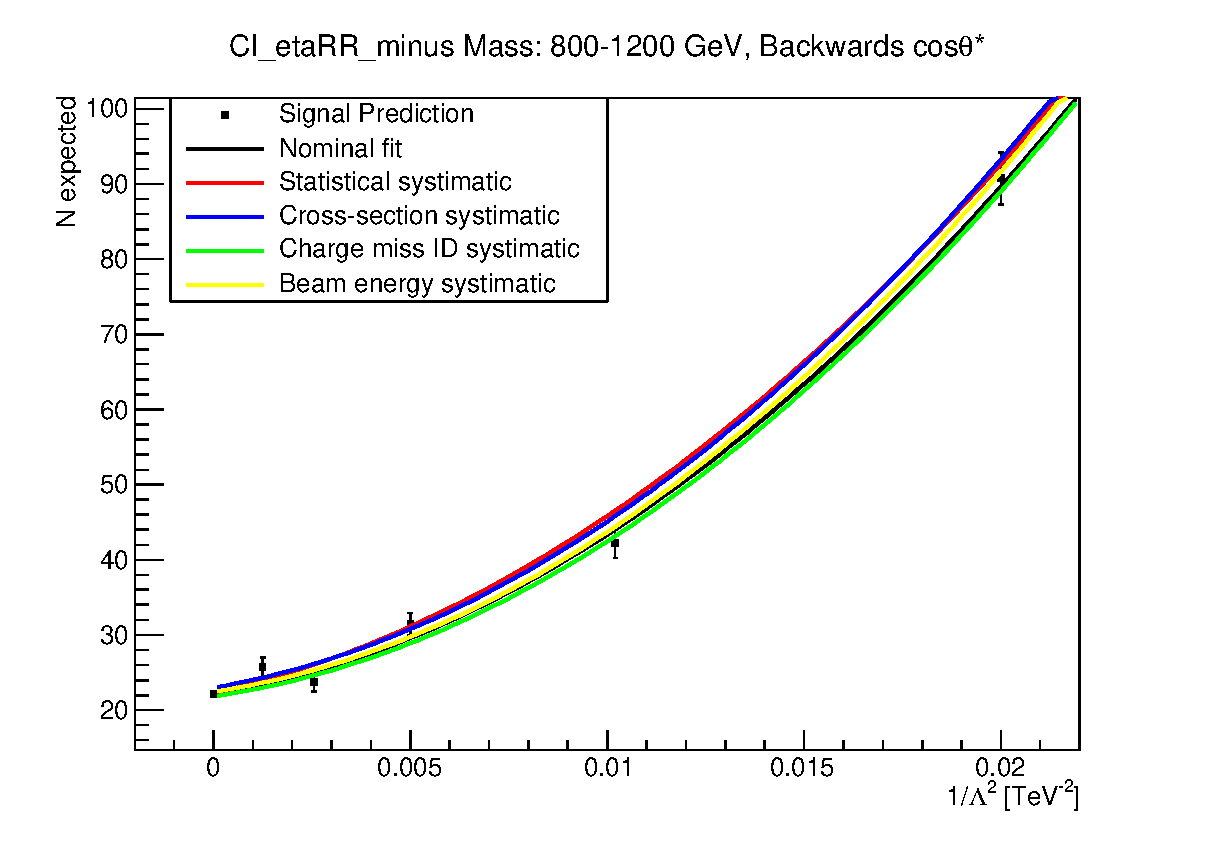
\includegraphics[width=0.49\linewidth]{images/thesis_fits/CI_2D_etaRR_minus_Mass_800-1200_GeV_CTS_-1_0.eps}
			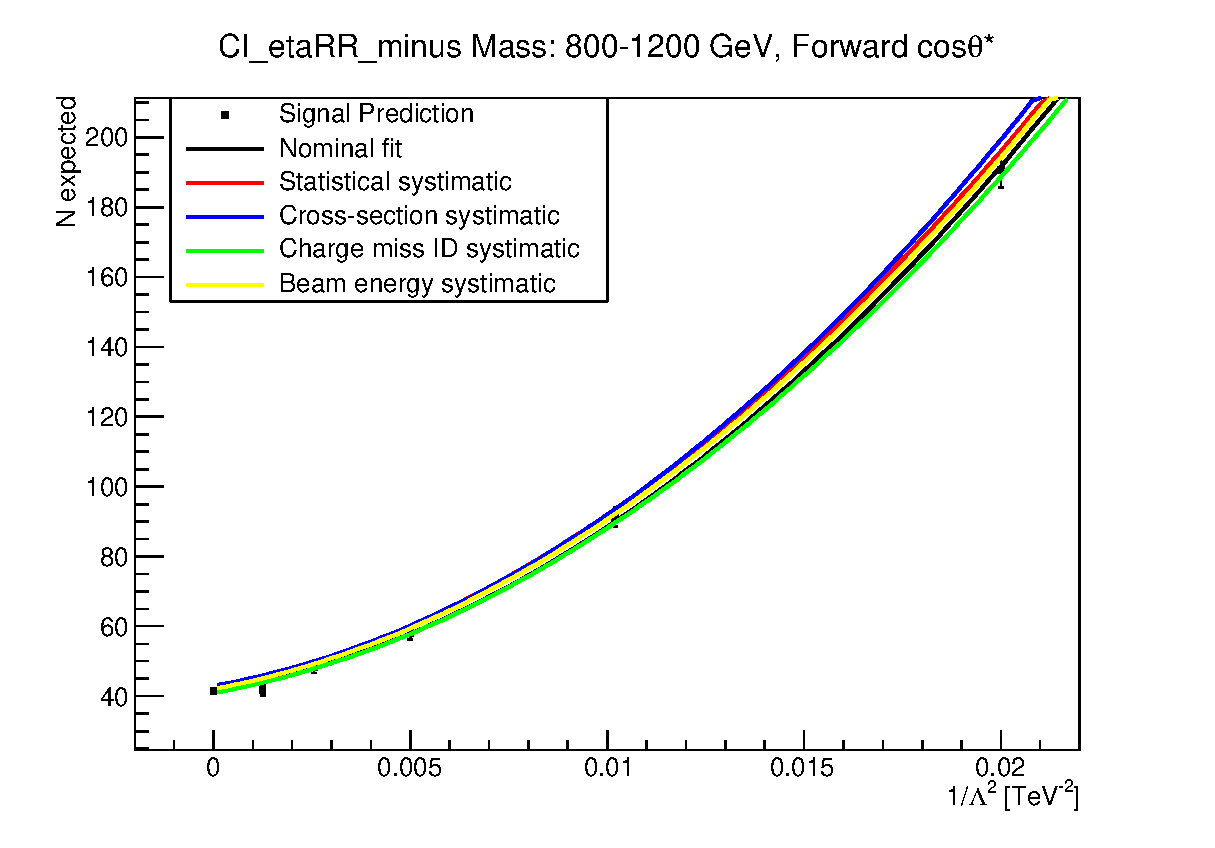
\includegraphics[width=0.49\linewidth]{images/thesis_fits/CI_2D_etaRR_minus_Mass_800-1200_GeV_CTS_0_1.eps}
		\caption{Signal paramaterisations for the RR formalism with constructive interferences for low mass bins}
		\label{fig:parm_RR_m_1}
	\end{figure}

	\begin{figure}[ht]
		\centering
			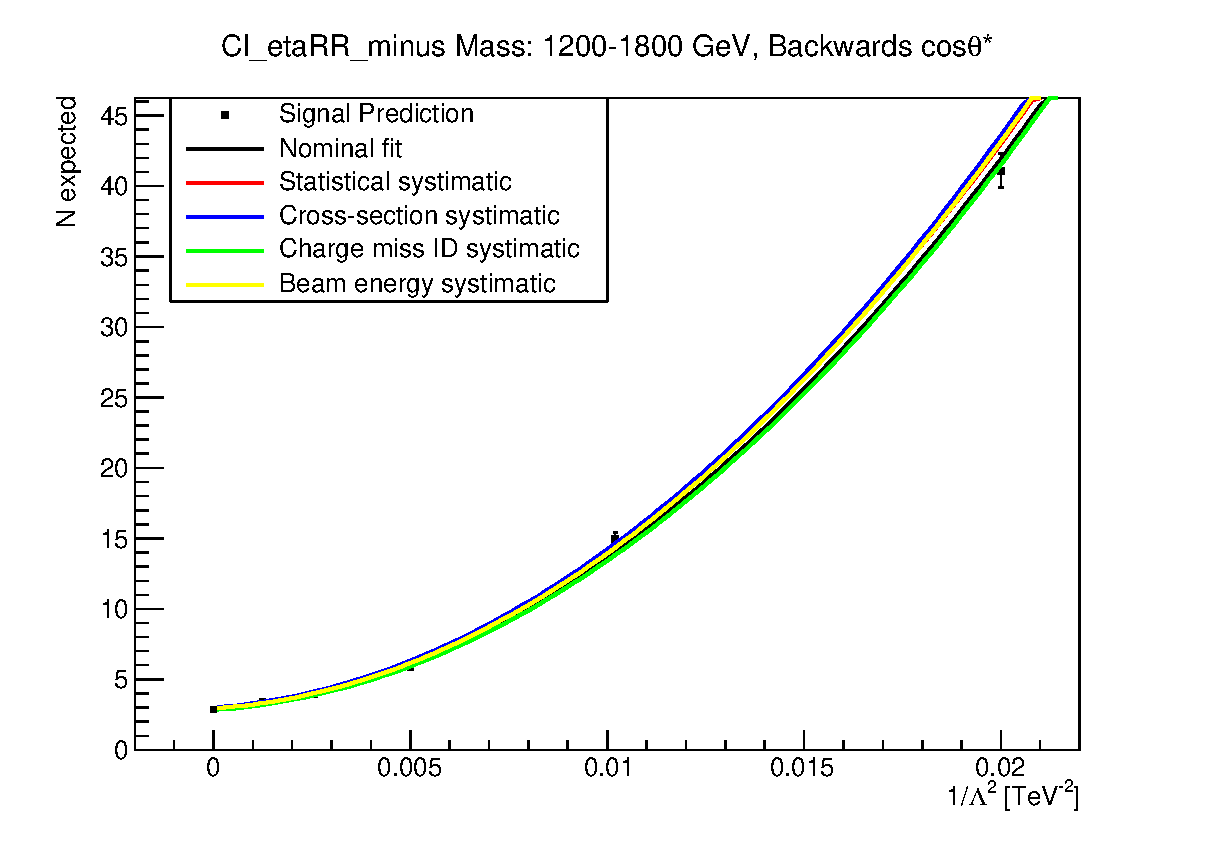
\includegraphics[width=0.49\linewidth]{images/thesis_fits/CI_2D_etaRR_minus_Mass_1200-1800_GeV_CTS_-1_0.eps}
			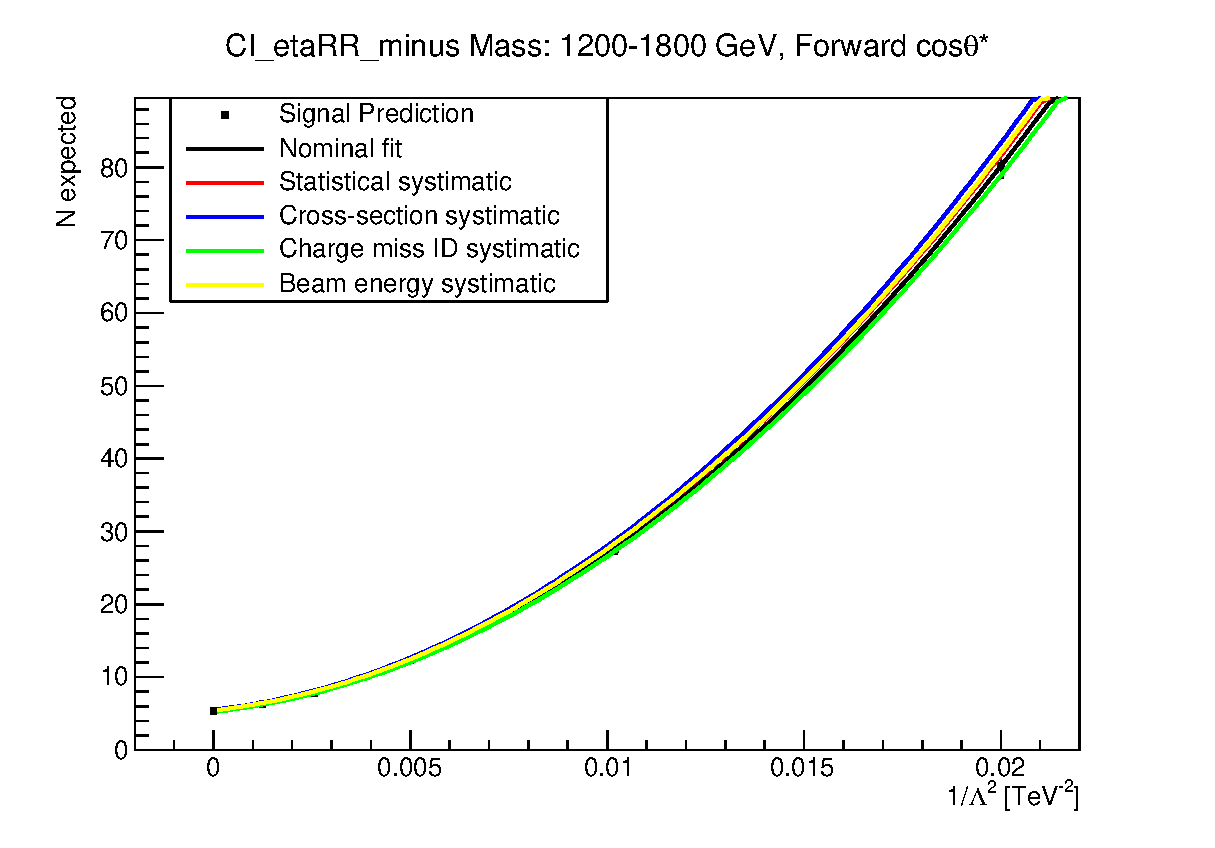
\includegraphics[width=0.49\linewidth]{images/thesis_fits/CI_2D_etaRR_minus_Mass_1200-1800_GeV_CTS_0_1.eps}
			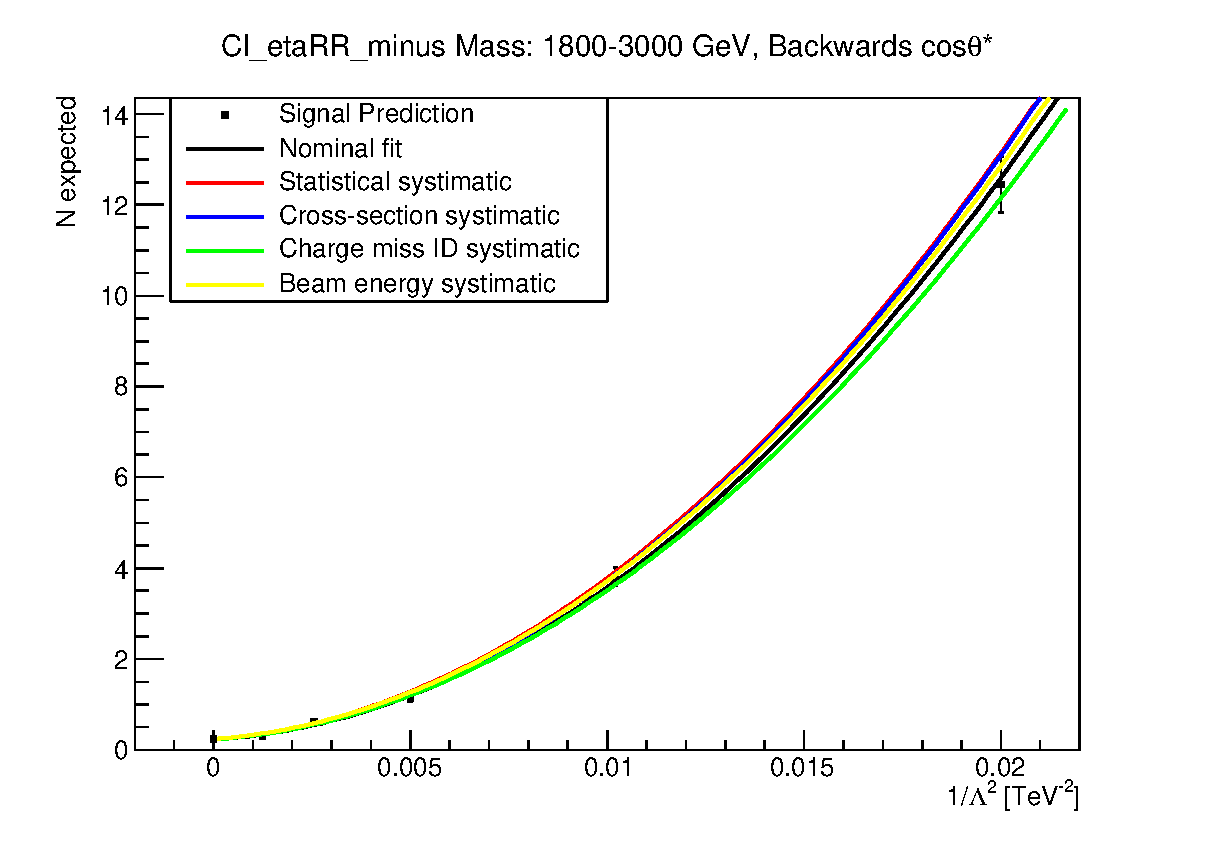
\includegraphics[width=0.49\linewidth]{images/thesis_fits/CI_2D_etaRR_minus_Mass_1800-3000_GeV_CTS_-1_0.eps}
			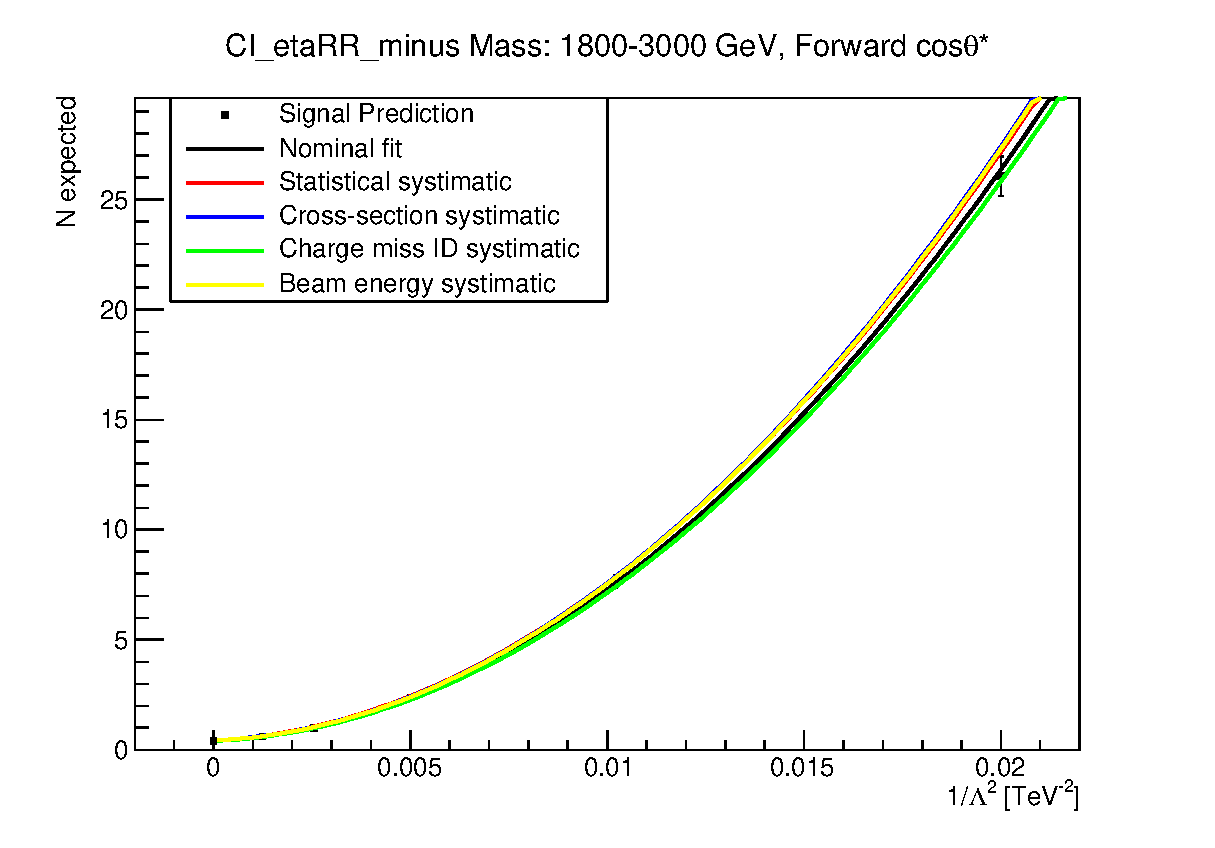
\includegraphics[width=0.49\linewidth]{images/thesis_fits/CI_2D_etaRR_minus_Mass_1800-3000_GeV_CTS_0_1.eps}
			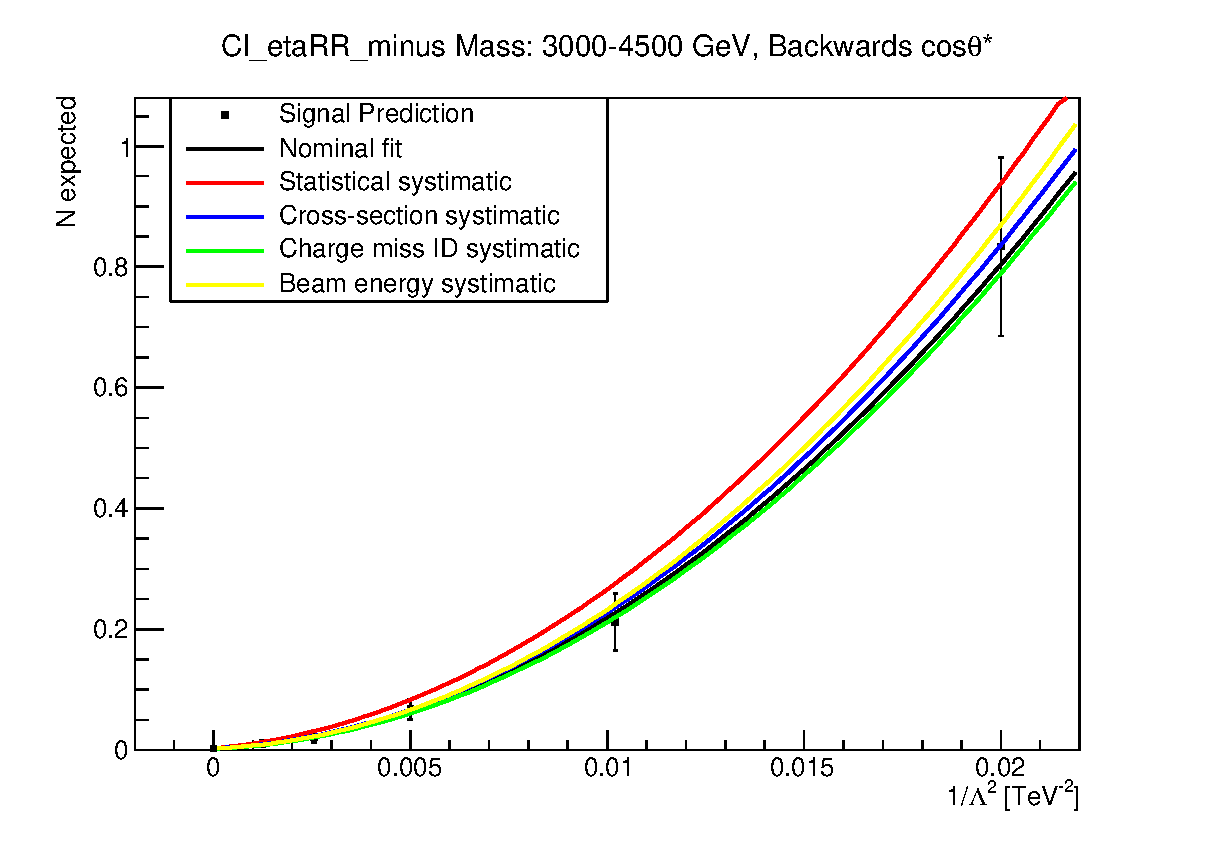
\includegraphics[width=0.49\linewidth]{images/thesis_fits/CI_2D_etaRR_minus_Mass_3000-4500_GeV_CTS_-1_0.eps}
			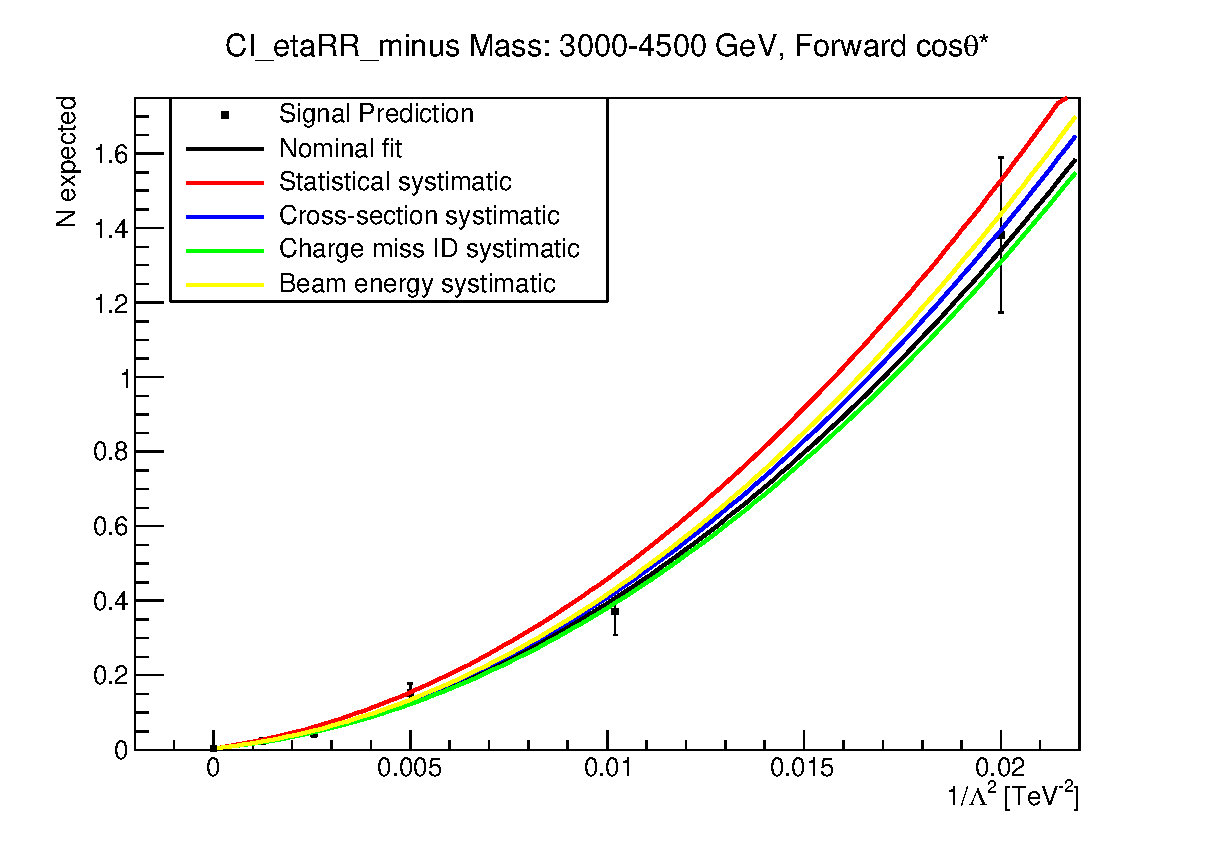
\includegraphics[width=0.49\linewidth]{images/thesis_fits/CI_2D_etaRR_minus_Mass_3000-4500_GeV_CTS_0_1.eps}
		\caption{Signal paramaterisations for the RR formalism with constructive interferences for high mass bins}
		\label{fig:parm_RR_m_2}
	\end{figure}


	\begin{figure}[ht]
		\centering
			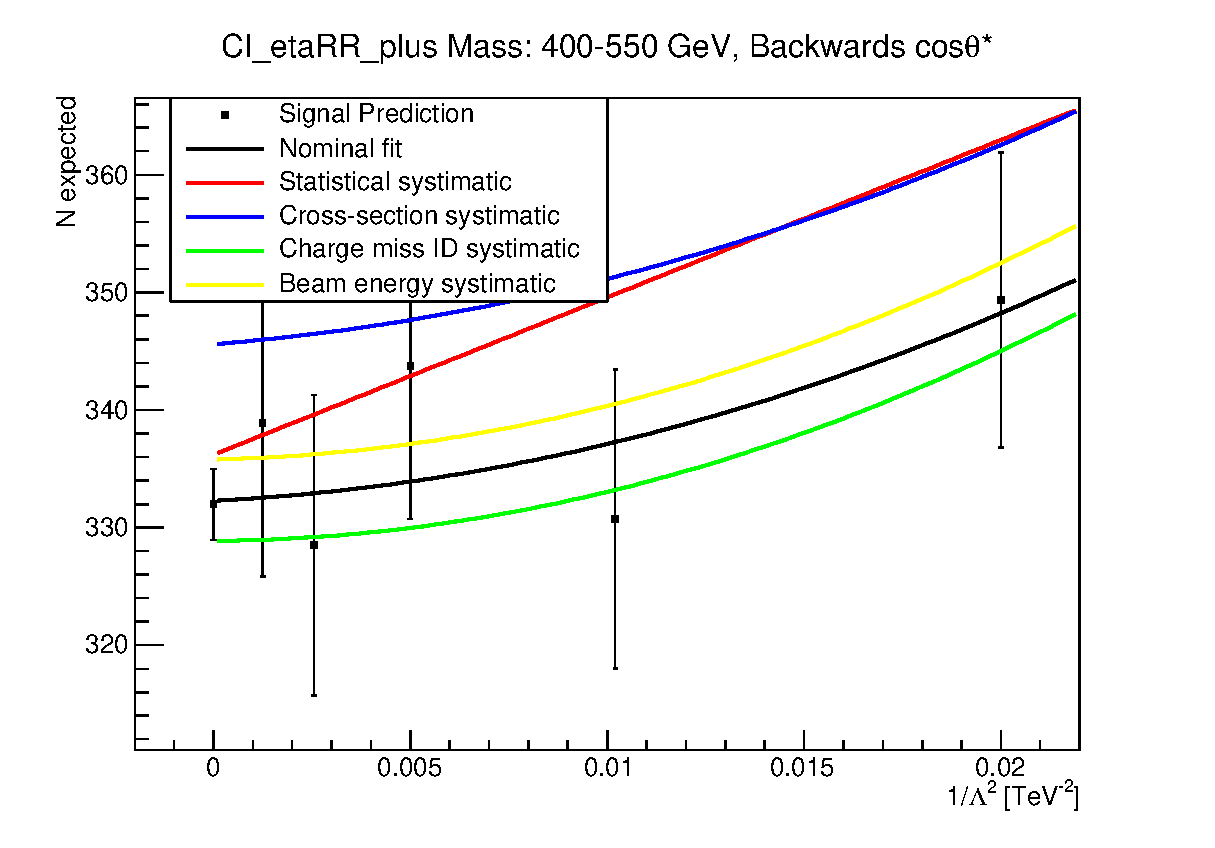
\includegraphics[width=0.49\linewidth]{images/thesis_fits/CI_2D_etaRR_plus_Mass_400-550_GeV_CTS_-1_0.eps}
			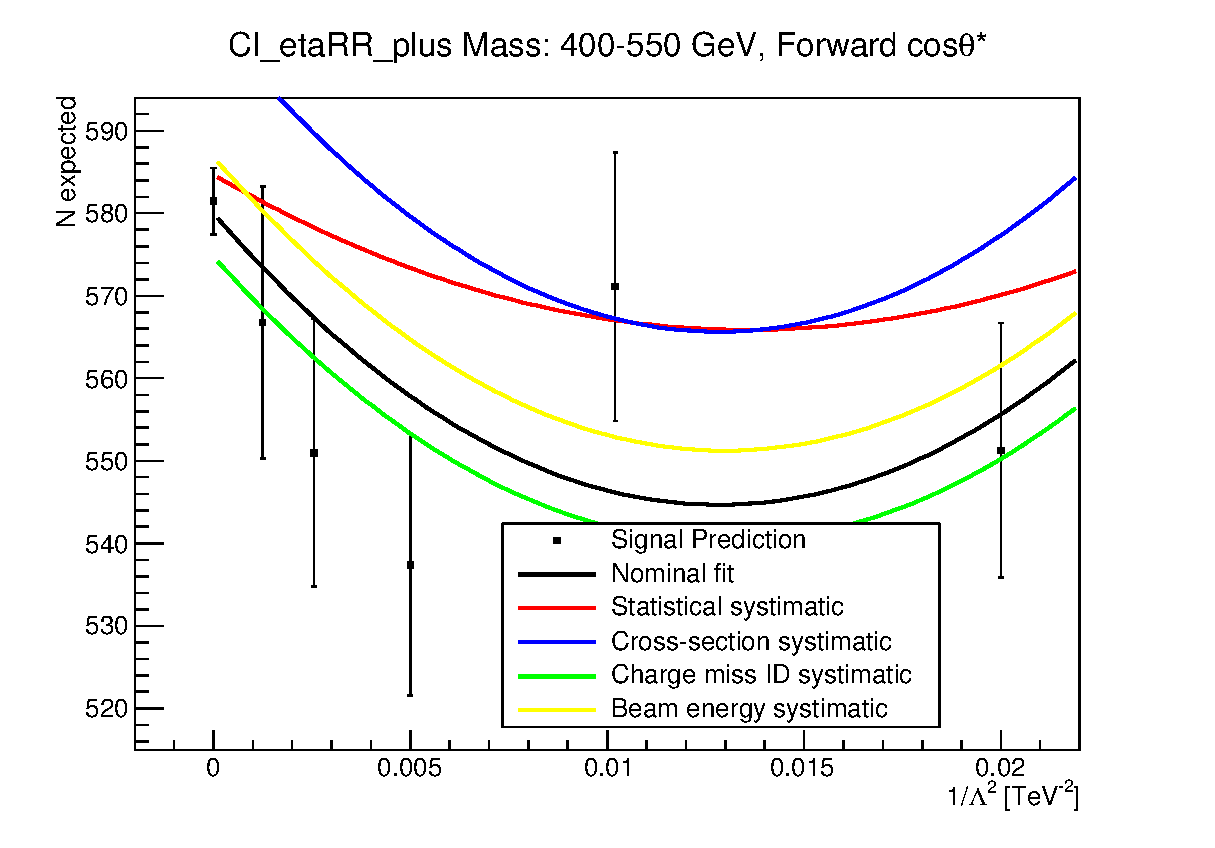
\includegraphics[width=0.49\linewidth]{images/thesis_fits/CI_2D_etaRR_plus_Mass_400-550_GeV_CTS_0_1.eps}
			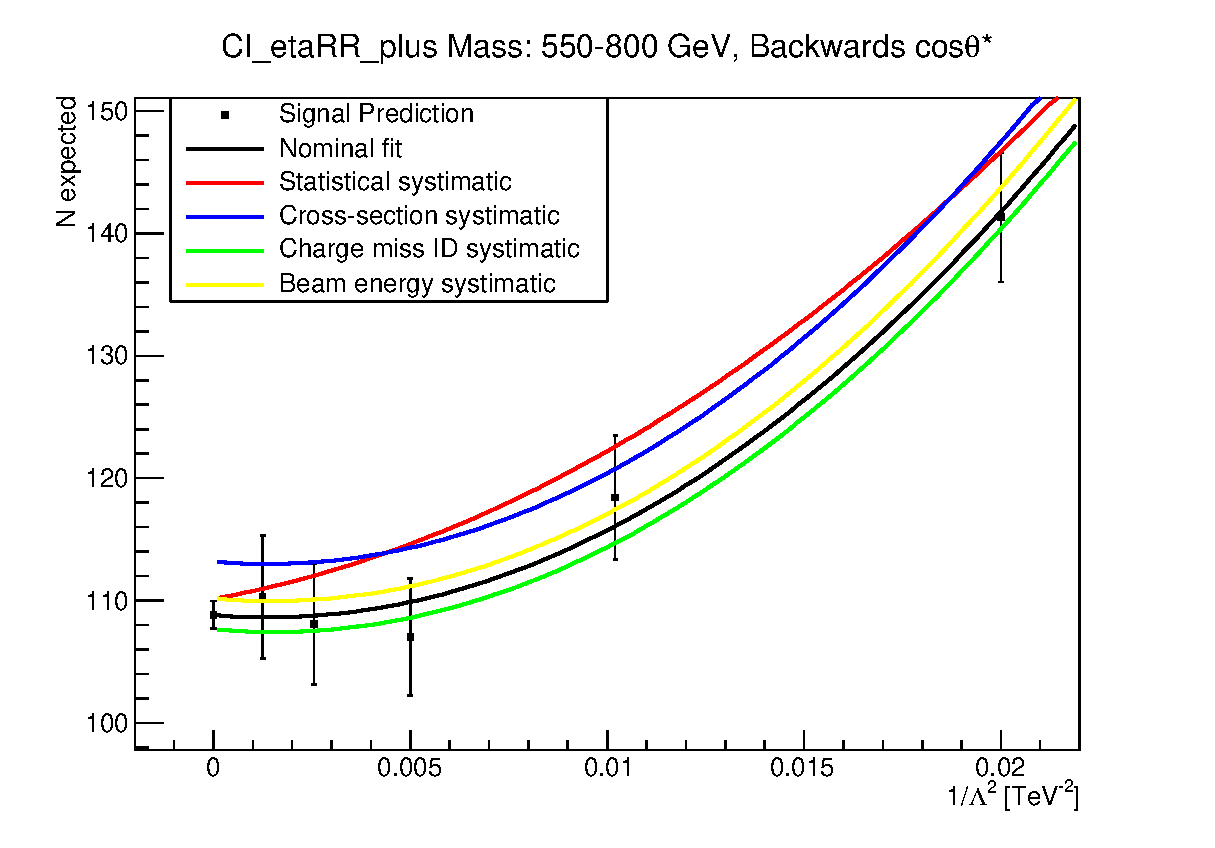
\includegraphics[width=0.49\linewidth]{images/thesis_fits/CI_2D_etaRR_plus_Mass_550-800_GeV_CTS_-1_0.eps}
			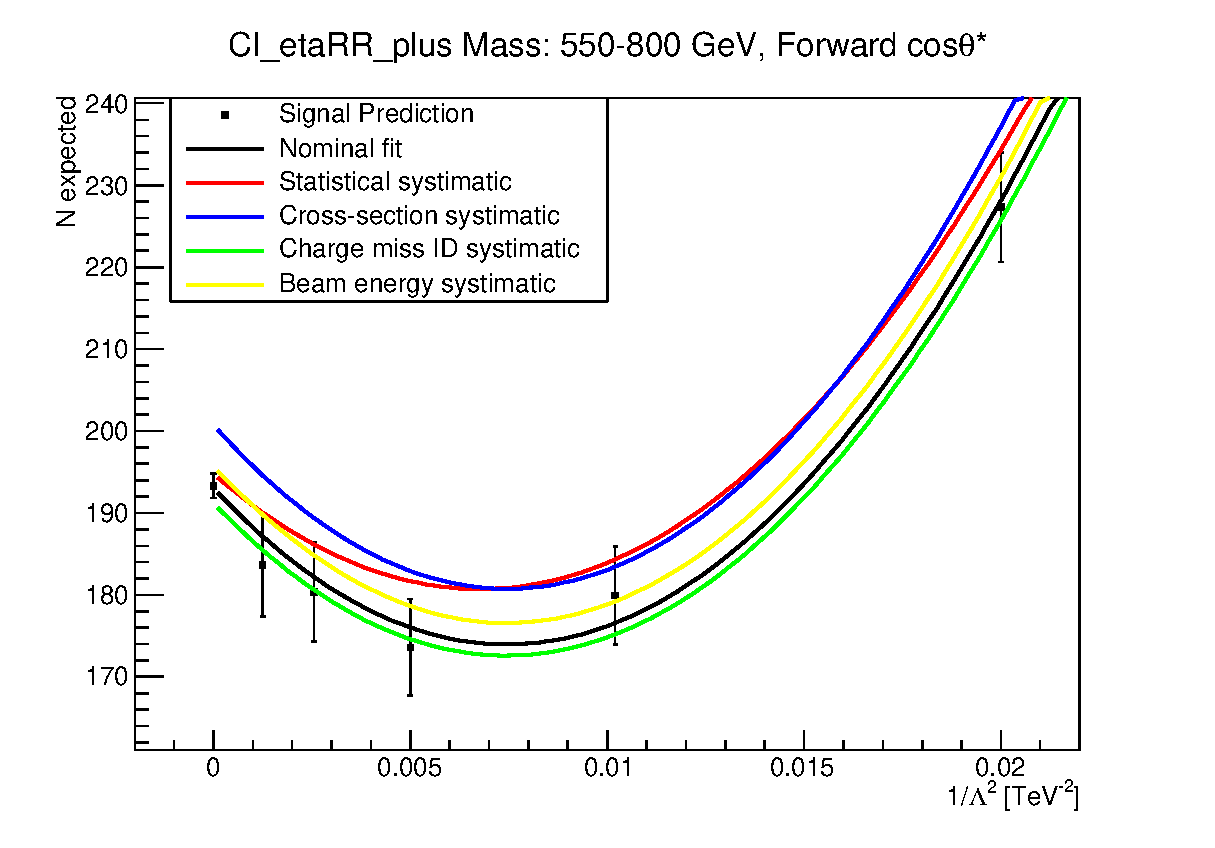
\includegraphics[width=0.49\linewidth]{images/thesis_fits/CI_2D_etaRR_plus_Mass_550-800_GeV_CTS_0_1.eps}
			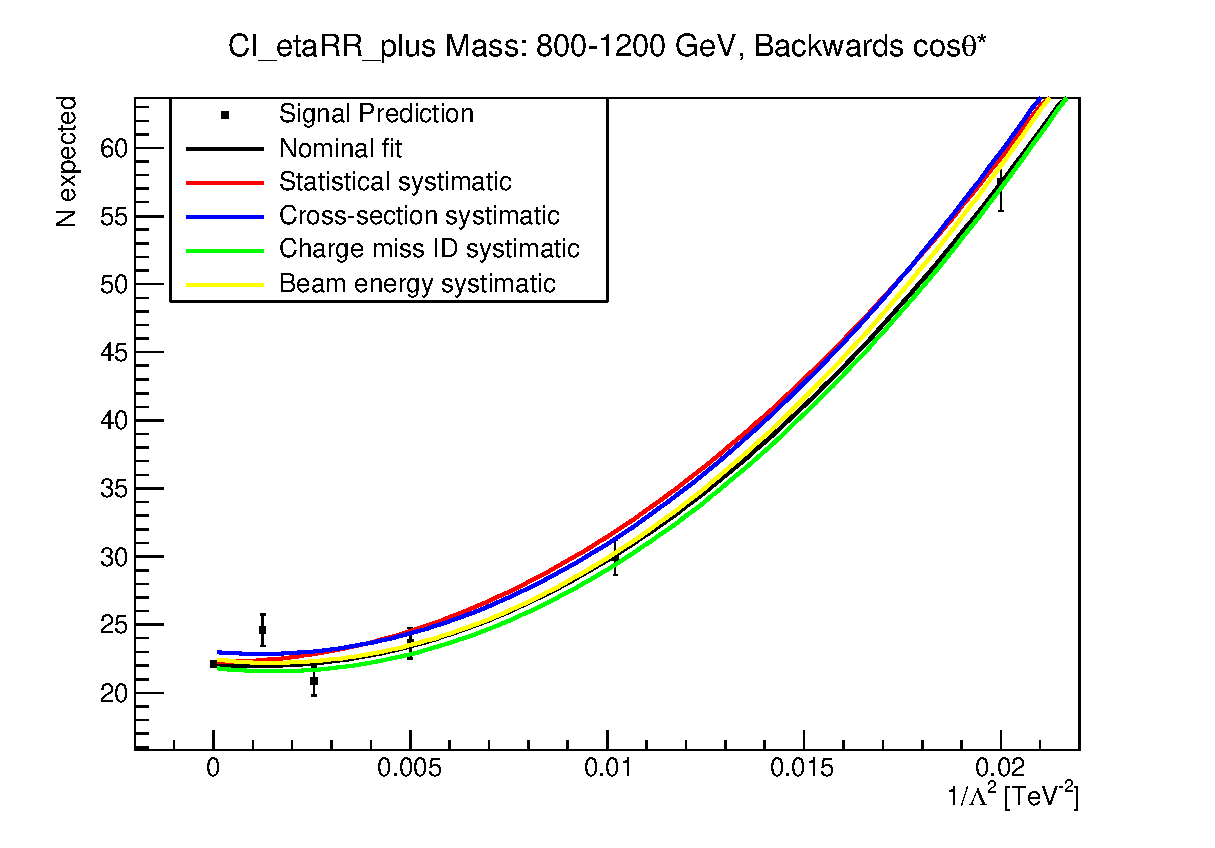
\includegraphics[width=0.49\linewidth]{images/thesis_fits/CI_2D_etaRR_plus_Mass_800-1200_GeV_CTS_-1_0.eps}
			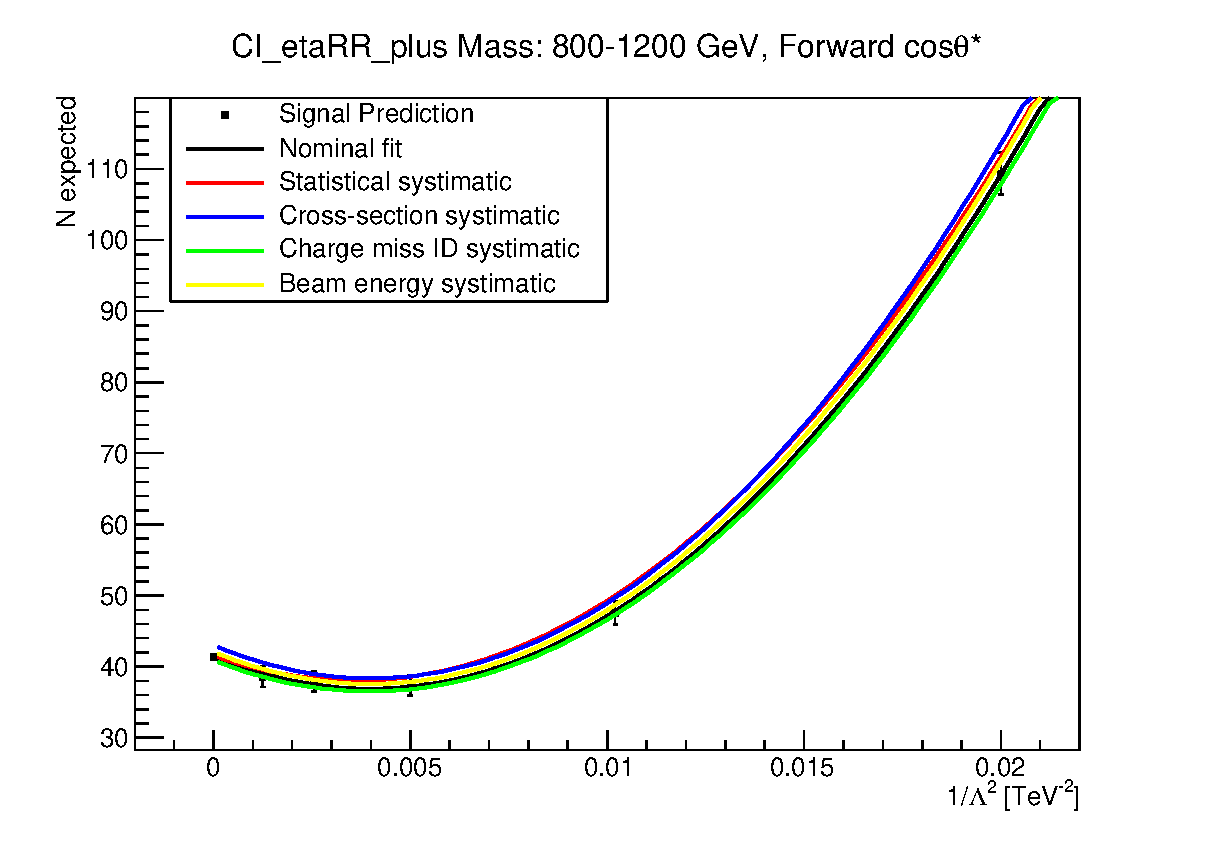
\includegraphics[width=0.49\linewidth]{images/thesis_fits/CI_2D_etaRR_plus_Mass_800-1200_GeV_CTS_0_1.eps}
		\caption{Signal paramaterisations for the RR formalism with destructive interferences for low mass bins}
		\label{fig:parm_RR_p_1}
	\end{figure}

	\begin{figure}[ht]
		\centering
			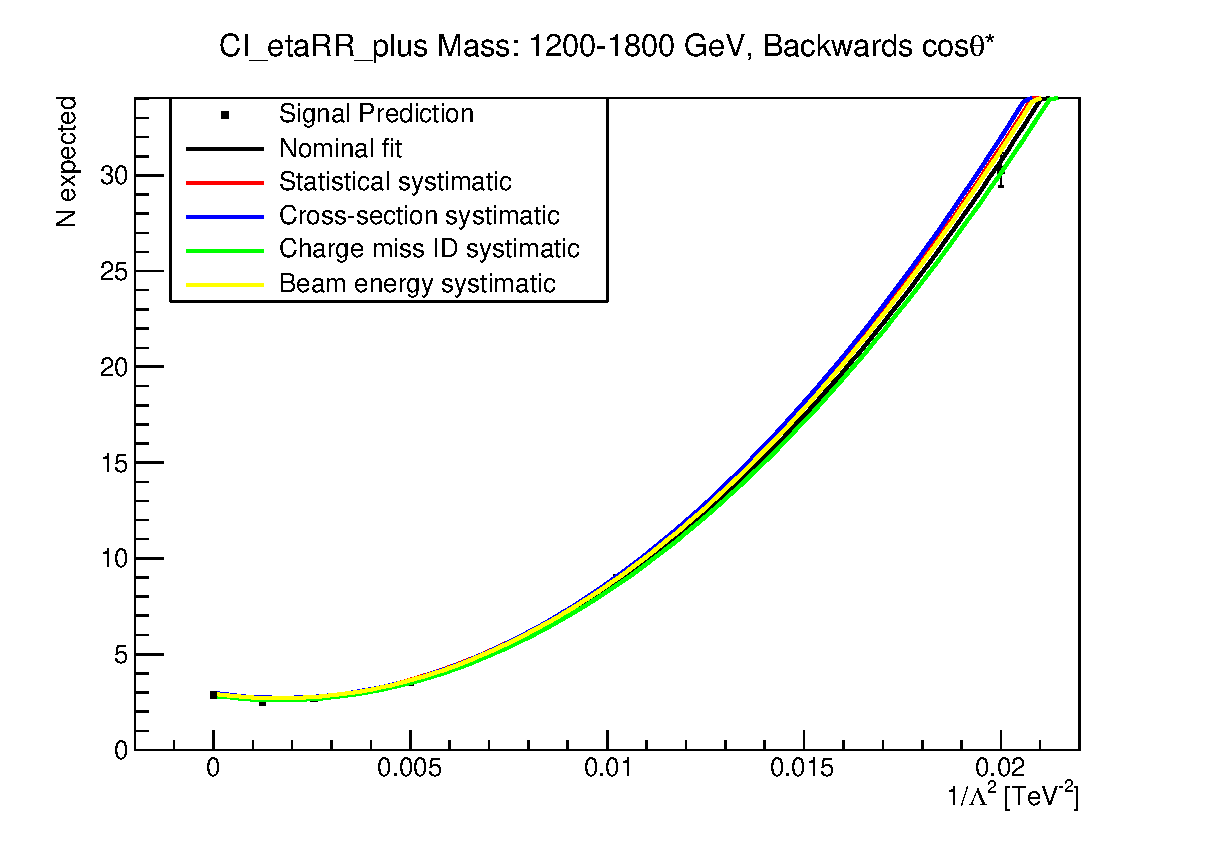
\includegraphics[width=0.49\linewidth]{images/thesis_fits/CI_2D_etaRR_plus_Mass_1200-1800_GeV_CTS_-1_0.eps}
			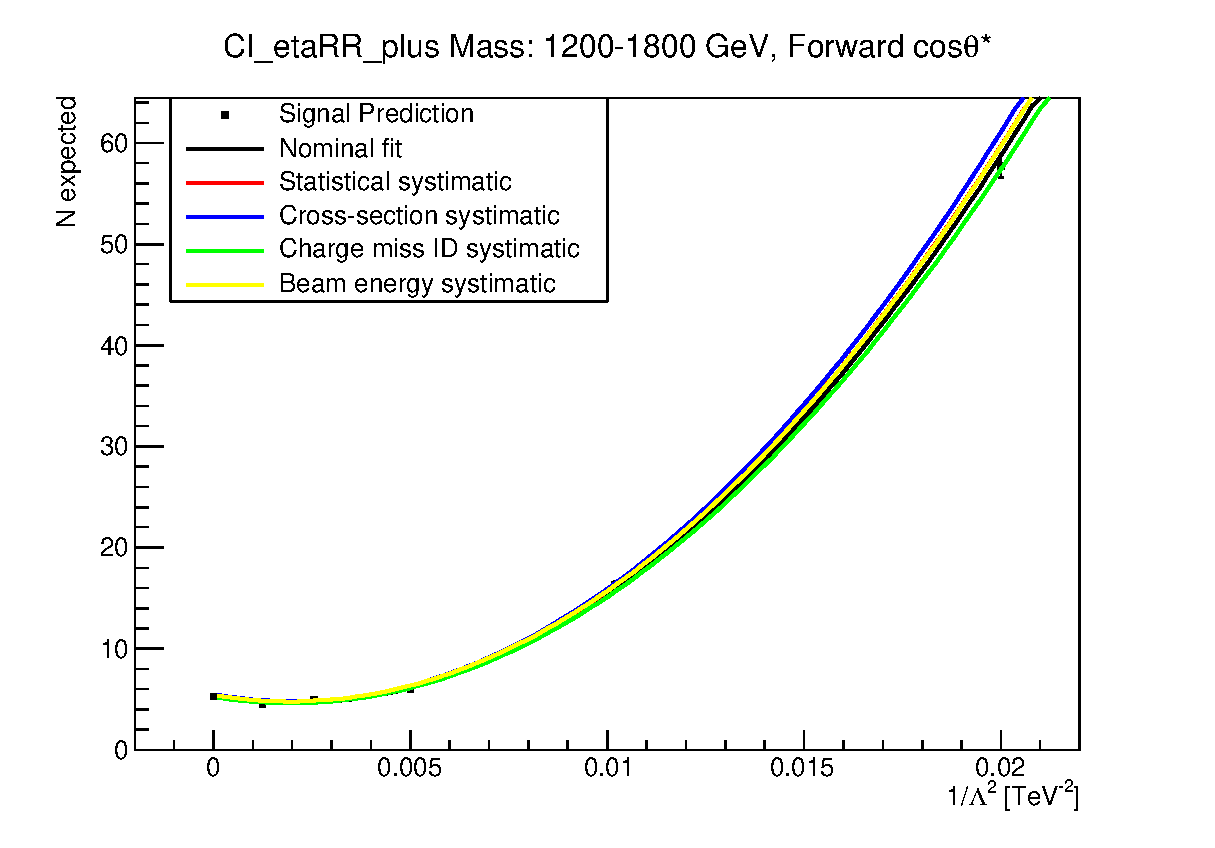
\includegraphics[width=0.49\linewidth]{images/thesis_fits/CI_2D_etaRR_plus_Mass_1200-1800_GeV_CTS_0_1.eps}
			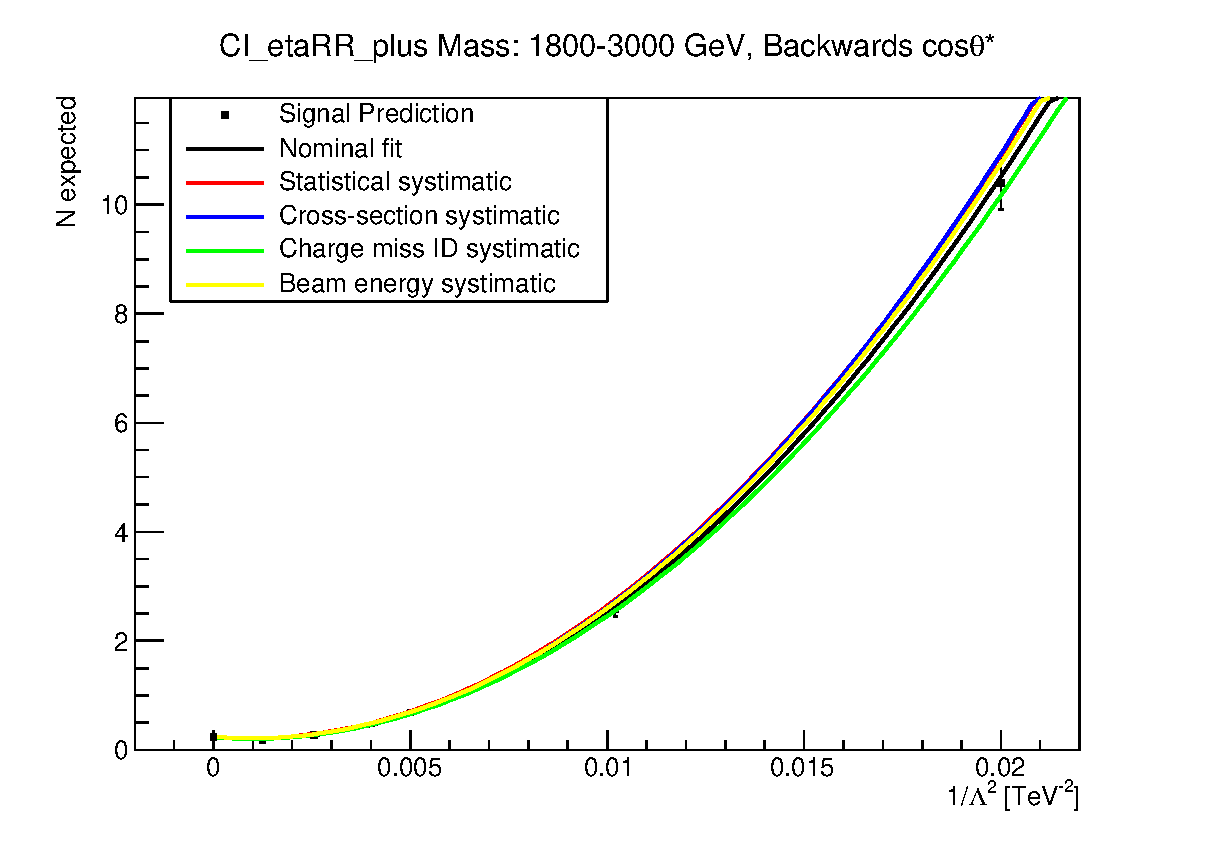
\includegraphics[width=0.49\linewidth]{images/thesis_fits/CI_2D_etaRR_plus_Mass_1800-3000_GeV_CTS_-1_0.eps}
			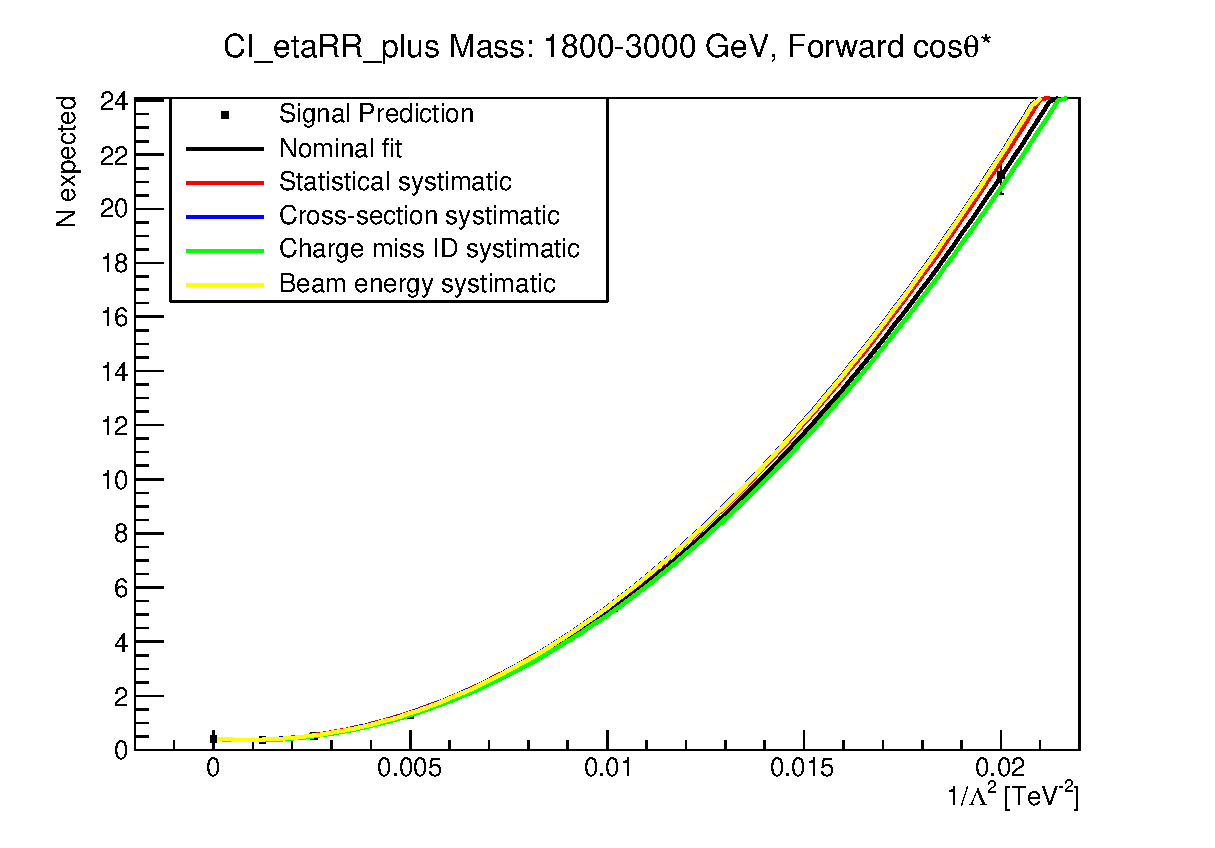
\includegraphics[width=0.49\linewidth]{images/thesis_fits/CI_2D_etaRR_plus_Mass_1800-3000_GeV_CTS_0_1.eps}
			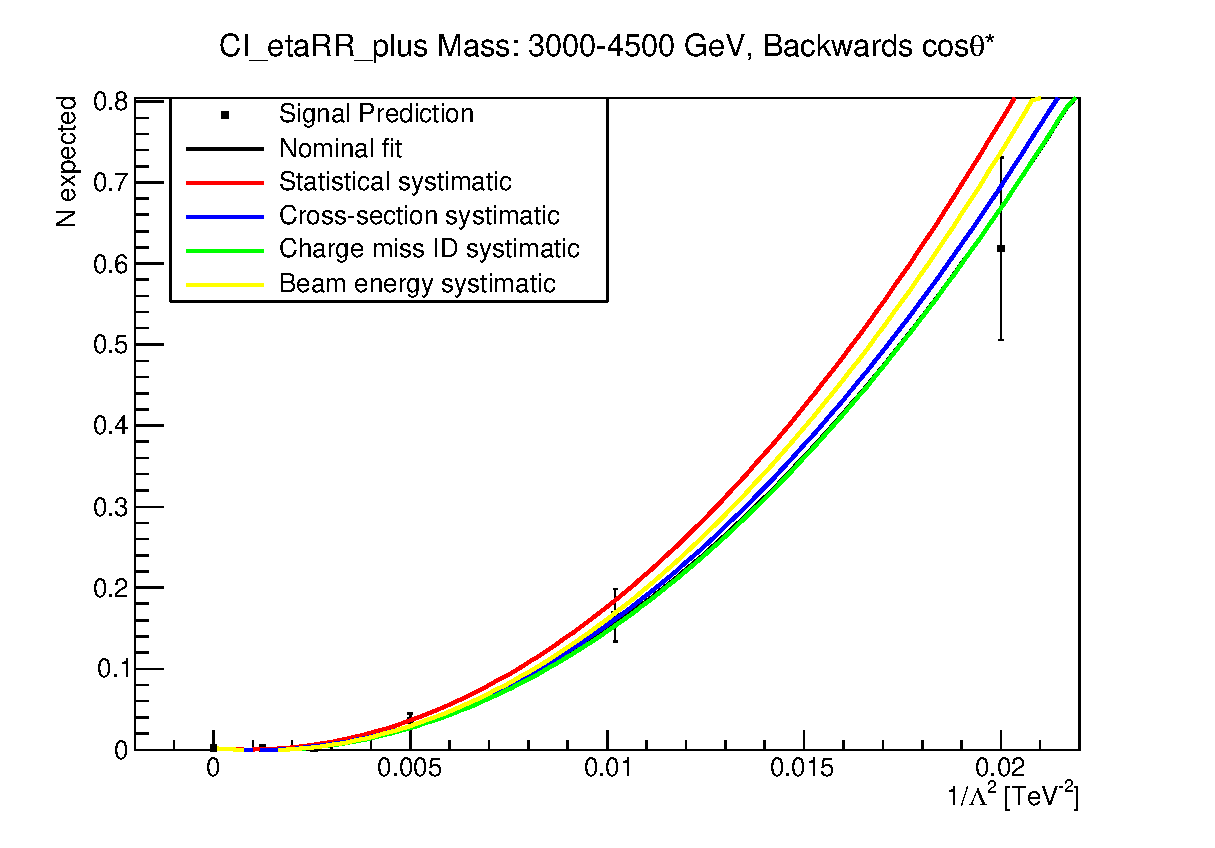
\includegraphics[width=0.49\linewidth]{images/thesis_fits/CI_2D_etaRR_plus_Mass_3000-4500_GeV_CTS_-1_0.eps}
			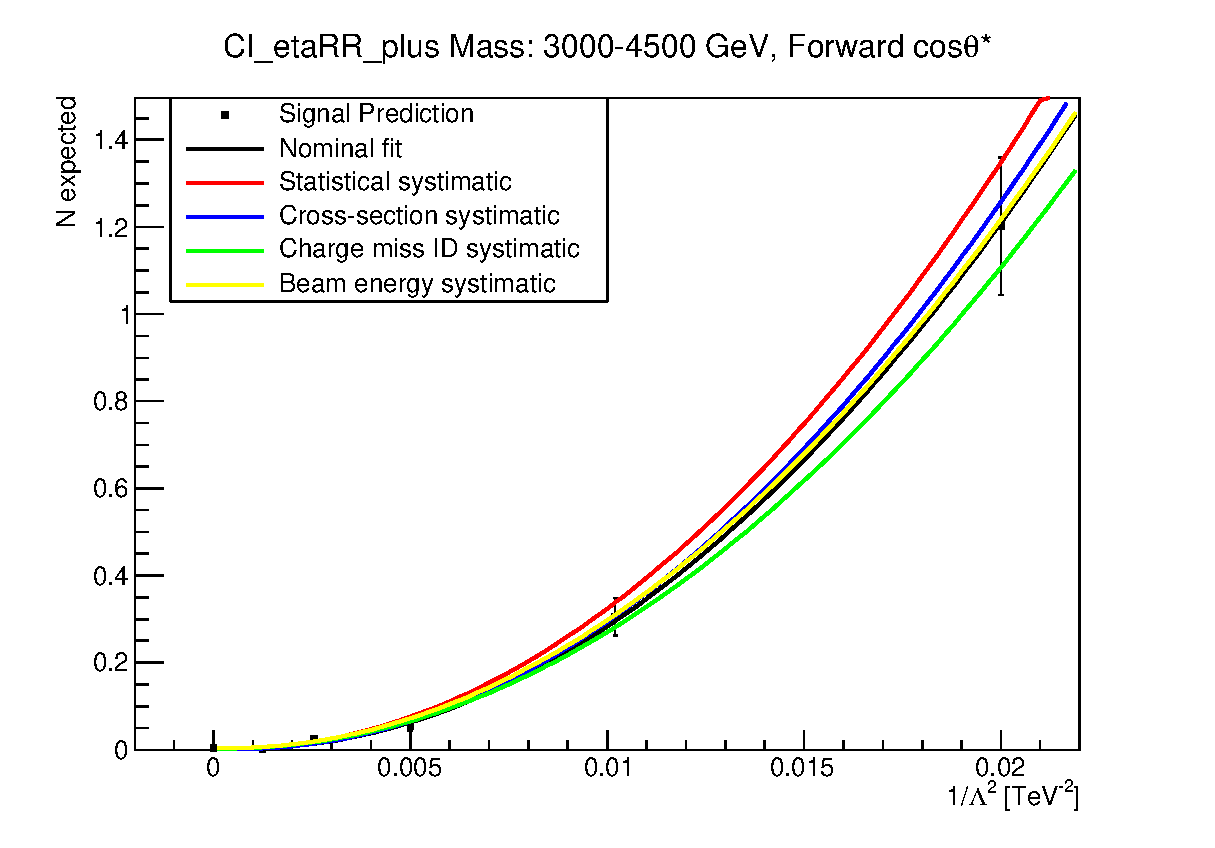
\includegraphics[width=0.49\linewidth]{images/thesis_fits/CI_2D_etaRR_plus_Mass_3000-4500_GeV_CTS_0_1.eps}
		\caption{Signal paramaterisations for the RR formalism with destructive interferences for high mass bins}
		\label{fig:parm_RR_p_2}
	\end{figure}
















	\begin{figure}[ht]
		\centering
			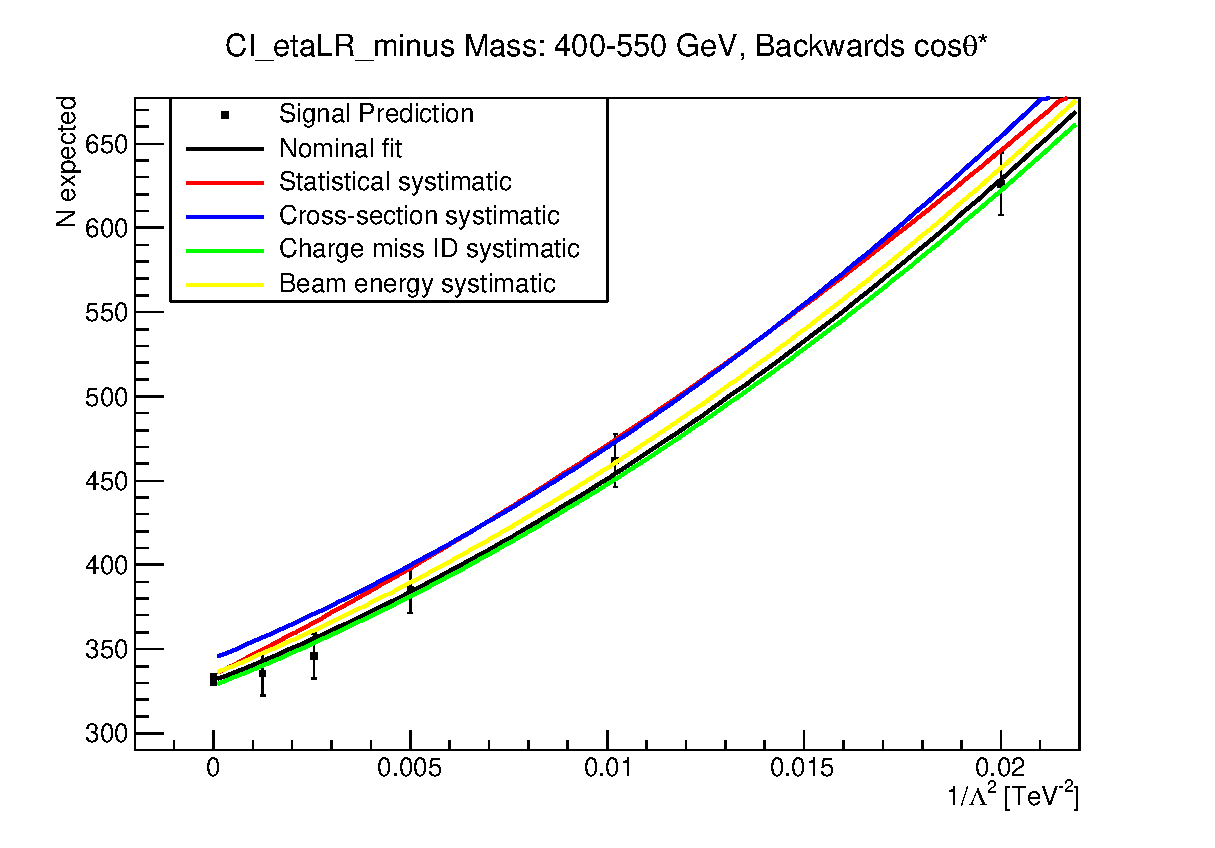
\includegraphics[width=0.49\linewidth]{images/thesis_fits/CI_2D_etaLR_minus_Mass_400-550_GeV_CTS_-1_0.eps}
			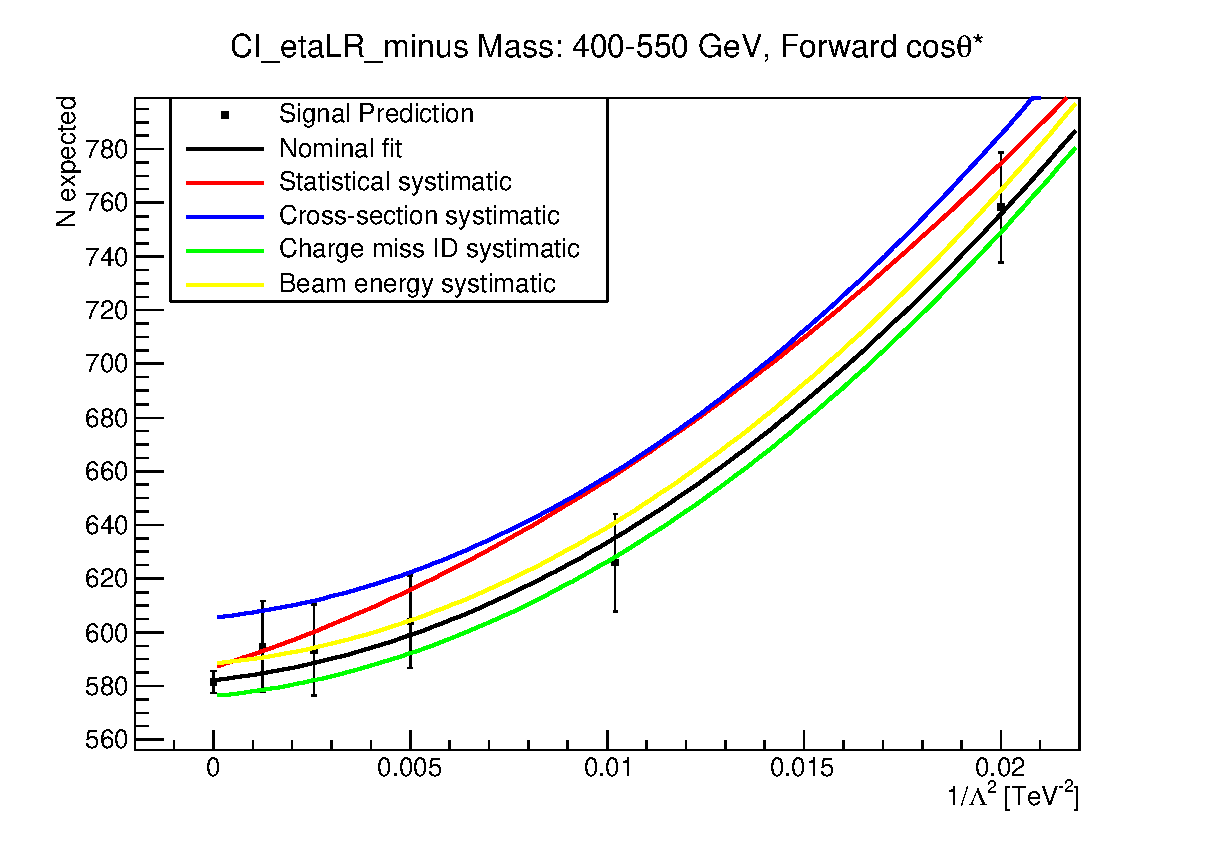
\includegraphics[width=0.49\linewidth]{images/thesis_fits/CI_2D_etaLR_minus_Mass_400-550_GeV_CTS_0_1.eps}
			\includegraphics[width=0.49\linewidth]{images/thesis_fits/CI_2D_etaLR_minus_Mass_550-800_GeV_CTS_-1_0.eps}
			\includegraphics[width=0.49\linewidth]{images/thesis_fits/CI_2D_etaLR_minus_Mass_550-800_GeV_CTS_0_1.eps}
			\includegraphics[width=0.49\linewidth]{images/thesis_fits/CI_2D_etaLR_minus_Mass_800-1200_GeV_CTS_-1_0.eps}
			\includegraphics[width=0.49\linewidth]{images/thesis_fits/CI_2D_etaLR_minus_Mass_800-1200_GeV_CTS_0_1.eps}
		\caption{Signal paramaterisations for the LR formalism with constructive interferences for low mass bins}
		\label{fig:parm_LR_m_1}
	\end{figure}

	\begin{figure}[ht]
		\centering
			\includegraphics[width=0.49\linewidth]{images/thesis_fits/CI_2D_etaLR_minus_Mass_1200-1800_GeV_CTS_-1_0.eps}
			\includegraphics[width=0.49\linewidth]{images/thesis_fits/CI_2D_etaLR_minus_Mass_1200-1800_GeV_CTS_0_1.eps}
			\includegraphics[width=0.49\linewidth]{images/thesis_fits/CI_2D_etaLR_minus_Mass_1800-3000_GeV_CTS_-1_0.eps}
			\includegraphics[width=0.49\linewidth]{images/thesis_fits/CI_2D_etaLR_minus_Mass_1800-3000_GeV_CTS_0_1.eps}
			\includegraphics[width=0.49\linewidth]{images/thesis_fits/CI_2D_etaLR_minus_Mass_3000-4500_GeV_CTS_-1_0.eps}
			\includegraphics[width=0.49\linewidth]{images/thesis_fits/CI_2D_etaLR_minus_Mass_3000-4500_GeV_CTS_0_1.eps}
		\caption{Signal paramaterisations for the LR formalism with constructive interferences for high mass bins}
		\label{fig:parm_LR_m_2}
	\end{figure}


	\begin{figure}[ht]
		\centering
			\includegraphics[width=0.49\linewidth]{images/thesis_fits/CI_2D_etaLR_plus_Mass_400-550_GeV_CTS_-1_0.eps}
			\includegraphics[width=0.49\linewidth]{images/thesis_fits/CI_2D_etaLR_plus_Mass_400-550_GeV_CTS_0_1.eps}
			\includegraphics[width=0.49\linewidth]{images/thesis_fits/CI_2D_etaLR_plus_Mass_550-800_GeV_CTS_-1_0.eps}
			\includegraphics[width=0.49\linewidth]{images/thesis_fits/CI_2D_etaLR_plus_Mass_550-800_GeV_CTS_0_1.eps}
			\includegraphics[width=0.49\linewidth]{images/thesis_fits/CI_2D_etaLR_plus_Mass_800-1200_GeV_CTS_-1_0.eps}
			\includegraphics[width=0.49\linewidth]{images/thesis_fits/CI_2D_etaLR_plus_Mass_800-1200_GeV_CTS_0_1.eps}
		\caption{Signal paramaterisations for the LR formalism with destructive interferences for low mass bins}
		\label{fig:parm_LR_p_1}
	\end{figure}

	\begin{figure}[ht]
		\centering
			\includegraphics[width=0.49\linewidth]{images/thesis_fits/CI_2D_etaLR_plus_Mass_1200-1800_GeV_CTS_-1_0.eps}
			\includegraphics[width=0.49\linewidth]{images/thesis_fits/CI_2D_etaLR_plus_Mass_1200-1800_GeV_CTS_0_1.eps}
			\includegraphics[width=0.49\linewidth]{images/thesis_fits/CI_2D_etaLR_plus_Mass_1800-3000_GeV_CTS_-1_0.eps}
			\includegraphics[width=0.49\linewidth]{images/thesis_fits/CI_2D_etaLR_plus_Mass_1800-3000_GeV_CTS_0_1.eps}
			\includegraphics[width=0.49\linewidth]{images/thesis_fits/CI_2D_etaLR_plus_Mass_3000-4500_GeV_CTS_-1_0.eps}
			\includegraphics[width=0.49\linewidth]{images/thesis_fits/CI_2D_etaLR_plus_Mass_3000-4500_GeV_CTS_0_1.eps}
		\caption{Signal paramaterisations for the LR formalism with destructive interferences for high mass bins}
		\label{fig:parm_LR_p_2}
	\end{figure}


